%Math template by Kaushik Srinivasan

\documentclass[11pt]{article}




%----------%
%  Basics  %
%----------%


%  Specfies basic information.
%  In the metadata section of the preamble, you can specify the subject and a list of keywords for the PDF.
%
\newcommand{\coursetitle}{AMS 553.430 - Introduction to Statistics}
\newcommand{\lecturer}{Dwijavanti P Athreya}
\newcommand{\notetaker}{Kaushik Srinivasan}
\newcommand{\notetakersemail}{ksriniv4@jhu.edu}
\newcommand{\courseterm}{Fall 2018}
\newcommand{\institution}{Johns Hopkins University}


%  array provides more column styles for the tabular and array environments.
%  (http://ctan.org/pkg/array)
%
%  parskip sets block paragraphs as the default, instead of indentation.
%  (http://www.ctan.org/pkg/parskip)
%
\usepackage[margin=1in]{geometry}
\usepackage{amsmath,amssymb,amsthm,amsfonts,array,parskip}


%  Allows equation, align, gather, etc. environments to split across pages.
\allowdisplaybreaks


%  Sets date formatting to the ISO 8601 standard, YYYY-MM-DD.
\usepackage{datetime} \renewcommand{\dateseparator}{-} \yyyymmdddate


%---------%
%  Fonts  %
%---------%


%  Defines \cal for standard calligraphy, \eucal for Euler calligraphy, and \frak for Fraktur.
\usepackage{eucal}  \let\eucal\mathcal  \let\cal\CMcal  \renewcommand{\frak}{\mathfrak}


%  Removes ligatures (e.g. the connection ordinarily made between the two f's in "differentiable").
%\usepackage{microtype} \DisableLigatures{encoding=*,family=*}


%  Removes extra space after periods.




%-------------------------------%
%  Environments and Sectioning  %
%-------------------------------%


%  Defines some standard theorem environments, in both numbered and non-numbered versions. The numbering of each enviroment will be reset for each lecture.
\newcounter{lecture}       \setcounter{lecture}{-1}
\newcounter{tN}[lecture]   \newcounter{dN}[lecture]
\newcounter{lN}[lecture]   \newcounter{rN}[lecture]
\newcounter{cN}[lecture]   \newcounter{eN}[lecture]
\newcounter{pN}[lecture]

\newtheorem*{theorem}{Theorem}          \newtheorem{theorem-N}[tN]{Theorem}
\newtheorem*{lemma}{Lemma}              \newtheorem{lemma-N}[lN]{Lemma}
\newtheorem*{corollary}{Corollary}      \newtheorem{corollary-N}[cN]{Corollary}
\newtheorem*{proposition}{Proposition}  \newtheorem{proposition-N}[pN]{Proposition}

\theoremstyle{definition}
\newtheorem*{definition}{Definition}    \newtheorem{definition-N}[dN]{Definition}
\newtheorem*{remark}{Remark}            \newtheorem{remark-N}[rN]{Remark}
\newtheorem*{example}{Example}          \newtheorem{example-N}[eN]{Example}
\newtheorem*{claim}{Claim}          \newtheorem{claim-N}[cN]{Claim}

\newtheorem*{question}{Question}
\newtheorem*{answer}{\emph{Answer}}

% Modifies the spacing above theorem environments, which is messed up during the parskip package

\makeatletter \def\thm@space@setup{\thm@preskip=\parskip \thm@postskip=0pt} \makeatother

%Modifies the spacing above the proof environment

\makeatletter \renewenvironment{proof}[1][\proofname]{\pushQED{\qed}\normalfont
\partopsep=\z@skip \topsep=\z@skip \trivlist \item[\hskip\labelsep\itshape #1\@addpunct{.}]
\ignorespaces}{\popQED\endtrivlist\@endpefalse} \makeatother

\renewcommand{\qedsymbol}{\rule{0.7em}{0.7em}}

%Removes extra space before and after section headings

\usepackage[compact]{titlesec}

%% PICTURES AND DIAGRAMS


\usepackage[usenames, dvipsnames]{xcolor}
\definecolor{myred}{rgb}{0.9,0.2,0.2}
\definecolor{mygreen}{rgb}{0.2,0.6,0.2}
\definecolor{myblue}{rgb}{0.2,0.2,0.8}
\usepackage{caption}

%graphicx provides advanced graphics options

\usepackage{graphicx}
\graphicspath{ {./images/} }

% tikz is for drawing all sorts of pictures and diagrams

\usepackage{tikz}
\usepackage{tabularx}
\usepackage{bbm}
\usetikzlibrary{decorations.text}
\newcommand{\tikzmark}[2]{%
    \tikz[remember picture,baseline=-2pt]
    \node[circle,red,draw,text=black,anchor=center,inner sep=1pt] (#1) {$#2$};}
\usepackage{tikz-cd}
\usepackage{pgf, pgfplots}
\usetikzlibrary{arrows,calc,decorations,decorations.markings,fadings,positioning,patterns,shapes}
\tikzset{>=latex}
\tikzstyle{mypoint}=[inner sep=0pt,outer sep=0pt,minimum size=5pt,fill,circle]
% for circled commands
\usepackage{enumitem}
%\begin{enumerate[label=\protect\circled{\arabic*}]
\newcommand*\circled[1]{\tikz[baseline=(char.base)]{\node[shape=circle,draw,inner sep=2pt] (char) {#1};}}

% HORIZONTAL LINES

\newcommand{\redhline}{\vspace{-0.1in}{\color{myred}{\rule{\textwidth}{0.02in}}}}


%------------------------%
%  Commands and Symbols  %
%------------------------%


%  Creates commands by running over a comma-separated list. For example,
%
%     \forcsvlist{\define{\newcommand}{\textbf}{bold}}{A,B}
%
%  would create
%
%     \newcommand{\boldA}{\textbf{A}}    \newcommand{\boldB}{\textbf{B}}
%
%  (http://tex.stackexchange.com/a/5776/20882)
%
\usepackage{etoolbox}
\newcommand{\define}[4]{\expandafter#1\csname#3#4\endcsname{#2{#4}}}
\forcsvlist{\define{\DeclareMathOperator}{}{}}{im,coker,rad,nil,Ann,Ass,codim,Spec,mSpec,diam,ord,Supp,supp,disc,Ob,vol,rank,Sym,Alt,Ind}
\forcsvlist{\define{\newcommand}{\mathrm}{}}{Hom,Mor,id,GL,SL,SO,SU,U,M,Mat,Ext,Tor,Res,Cor,Inf,End,Irr,Aut,Gal,lcm,tr,sign,triv,diag,Map,op,ev,act,alg,sep,unr,nr,ab}

%  Creates commands for some names of categories in the sans-serif font.
\forcsvlist{\define{\newcommand}{\mathsf}{}}{Set,Grp,Ab,CRing,Mod,Vect,Cat,Top,PreSh,Sh,Sch,Nat,Fun,Diff}

%  Creates commands for some blackboard bold letters.
\forcsvlist{\define{\newcommand}{\mathbb}{}}{N,Z,Q,R,C,F,G,T,A,B,D}
\newcommand{\Rn}{\mathbb{R}}
\newcommand{\bX}{\bar{X}}
\newcommand{\ux}{\underline{x}}
\newcommand{\uX}{\underline{X}}

%  Saves the section symbol, paragraph symbol, Hungarian accent, and Scandanavian O in the macros \SS, \PP, \HH, and \OO, then redefines \S, \P, \H, and \O to be the corresponding blackboard bold letters.
%
\let\SS\S  \let\PP\P  \let\HH\H  \let\OO\O
\forcsvlist{\define{\renewcommand}{\mathbb}{}}{S,P,H,O}


%  latexsym defines some alternative versions of amssymb symbols.
%  (http://www.bakoma-tex.com/doc/latex/base/latexsym.pdf)
%
\usepackage{latexsym}

\usepackage{accents}
\newcommand{\Ylines}{\underaccent{\bar}{\bar{Y}}}
\newcommand{\Xlines}{\underaccent{\bar}{\bar{X}}}
\newcommand{\Lim}[1]{\raisebox{0.5ex}{\scalebox{0.8}{$\displaystyle \lim_{#1}\;$}}}
%  Defines a copyright symbol that is a bit nicer than the built-in one.
\newcommand{\mycopyrightsymbol}{\raisebox{-0.3ex}{\tikz{\node[inner sep=0pt,outer sep=0pt] at (0,0) {\textsc{c}};\draw (0,0) circle (0.18);}}}


%  Defines commands for real and complex projective space.
\newcommand{\RP}{\mathbb{R}\mathrm{P}}  \newcommand{\CP}{\mathbb{C}\mathrm{P}}


%  Defines a bordered matrix with square bracket delimiters instead of parentheses.
%  (http://tex.stackexchange.com/questions/55054)
%
\let\bbordermatrix\bordermatrix
\patchcmd{\bbordermatrix}{8.75}{4.75}{}{}
\patchcmd{\bbordermatrix}{\left(}{\left[}{}{}
\patchcmd{\bbordermatrix}{\right)}{\right]}{}{}

%% MATH STUFF

\usepackage{relsize}
\usepackage{cancel}

%Box Colour (https://tex.stackexchange.com/questions/122945/coloured-shadowed-boxes-around-equations)
\usepackage[skins,theorems]{tcolorbox}
\usepackage{tcolorbox}
\tcbset{highlight math style={enhanced, colframe=red,colback=white,arc=0pt,boxrule=1pt}}
  


% Math Symbol Aliases

\newcommand{\bs}{\backslash}
\newcommand{\subeq}{\subseteq}
\newcommand{\supeq}{\supseteq}
\newcommand{\subneq}{\subsetneq}
\newcommand{\supneq}{\supsetneq}
\newcommand{\derivativex}{\dfrac{\partial}{\partial x}}
\newcommand{\customderiv}[2]{\dfrac{\partial #1}{\partial #2}}


% Accents

\newcommand{\openset}{\,\open{\subeq}\,}
\newcommand{\open}[1]{\mathring{#1}}
\newcommand{\clos}[1]{\overline{#1}}
\newcommand{\resid}[1]{\overline{#1}}
\newcommand{\cover}[1]{\widetilde{#1}}
\newcommand{\overbar}[1]{%
  \mkern 1.5mu\overline{\mkern-1.5mu#1\mkern-1.5mu}\mkern 1.5mu%
}

%  Defines a bordered matrix with square bracket delimiters instead of parentheses.
%  (http://tex.stackexchange.com/questions/55054)
%
\let\bbordermatrix\bordermatrix
\patchcmd{\bbordermatrix}{8.75}{4.75}{}{}
\patchcmd{\bbordermatrix}{\left(}{\left[}{}{}
\patchcmd{\bbordermatrix}{\right)}{\right]}{}{}

%  Calls one of the mathabx font families so that it is possible to use its symbols without making a global change.
%  (http://www.ctan.org/pkg/mathabx)
%  (http://tex.stackexchange.com/questions/14386)
%
\DeclareFontFamily{U}{mathb}{\hyphenchar\font45}
\DeclareFontShape{U}{mathb}{m}{n}{<5> <6> <7> <8> <9> <10> gen * mathb
<10.95> mathb10 <12> <14.4> <17.28> <20.74> <24.88> mathb12}{}
\DeclareSymbolFont{mathb}{U}{mathb}{m}{n}

% Defines circular arrows

\DeclareFontFamily{U}{mathb}{\hyphenchar\font45}
\DeclareFontShape{U}{mathb}{m}{n}{<5> <6> <7> <8> <9> <10> gen * mathb
<10.95> mathb10 <12> <14.4> <17.28> <20.74> <24.88> mathb12}{}
\DeclareSymbolFont{mathb}{U}{mathb}{m}{n}

%  Defines circular arrows.
\DeclareMathSymbol{\lcirclearrow}{0}{mathb}{'366}
\DeclareMathSymbol{\rcirclearrow}{0}{mathb}{'367}
\newcommand{\leftcirclearrow}{\mathrel{\ensuremath{\raisebox{0.1ex}{\scalebox{0.9}{\rotatebox[origin=c]{90}{$\lcirclearrow$}}}}}}
\newcommand{\rightcirclearrow}{\mathrel{\ensuremath{\raisebox{0.1ex}{\scalebox{0.9}{\rotatebox[origin=c]{270}{$\rcirclearrow$}}}}}}

% Semantic names for some common math Symbols.

%-----------------------------------%
%  Things Specific to Course Notes  %
%-----------------------------------%


%  Formatting for the table of contents. The first line allows for multi-column environments, the second line removes the heading "Contents".
\usepackage{multicol} \setlength{\columnsep}{3cm}
\makeatletter \renewcommand\tableofcontents{\@starttoc{toc}} \makeatother


%  Sets the page style.
\usepackage{fancyhdr}
\pagestyle{fancy}
\renewcommand{\headrulewidth}{0pt}
\renewcommand{\footrulewidth}{0.5pt}
\setlength{\headheight}{14pt}
\lfoot{\parbox[t]{1in}{\centering Last edited\\ \today}}
\cfoot{\parbox[t]{3in}{\centering \coursetitle}}
\rfoot{\parbox[t]{0.9in}{\centering Page \thepage\\ Lecture \arabic{lecture}}}


%  Sets the inputs for \maketitle.
\author{Lectures by \lecturer\\ Notes by \notetaker}
\title{\coursetitle}
\date{\institution\\ \courseterm}


%  Defines headings for each day's notes.
\newcommand{\classheader}[1]{\stepcounter{lecture}\newpage\section*{Lecture \arabic{lecture} (#1)}
\phantomsection \addcontentsline{toc}{section}{Lecture \arabic{lecture} (#1)}}
	
% Misc additions to Template

% http://tex.stackexchange.com/questions/18359
\pgfplotsset{compat=newest}

\newcommand{\Cinfty}{\ensuremath{C^{\infty}}}
\newcommand{\Crit}{\mathrm{Crit}}
\usepackage{mathtools}
\newcommand{\Or}{\mathrm{Or}}
\renewcommand{\Re}{\mathrm{Re}}
\renewcommand{\Im}{\mathrm{Im}}
\usepackage{mathrsfs}
\newtheorem*{examples}{Examples}
\newtheorem*{exercise}{Exercise}
\usepackage{pdfpages}
\newcommand{\Lie}{\mathrm{Lie}}
\newcommand{\Diffeo}{\mathrm{Diffeo}}

\newcommand*{\Perm}[2]{{}^{#1}\!P_{#2}}%
\newcommand*{\Comb}[2]{{}^{#1}C_{#2}}%

\newcommand{\connection}{\nabla}
\newcommand{\new}{\mathrm{new}}


\newcommand{\review}{{\huge\color{myred}{$\star$}}}


%---------------------------%
%  Hyperlinks and Metadata  %
%---------------------------%
%
% (this section must come last!)


%  hyperref enables for the creation of hyperlinks, and also specifies the metadata of the PDF file.
%  hyperxmp allows more metadata to be specified.
%  (http://www.ctan.org/pkg/hyperref)
%  (http://www.ctan.org/pkg/hyperxmp)
%  (http://tex.stackexchange.com/questions/41461)
%
\usepackage{hyperref}
\usepackage{hyperxmp}
\hypersetup{
pdfauthor={\notetaker},
pdftitle={\coursetitle},
pdfproducer={LaTeX},
%pdfcopyright={Copyright (C) \the\year\ \notetaker. This work is licensed under a Creative Commons Attribution-ShareAlike 3.0 Unported License. All attribution should be to \lecturer\ as the lecturer, and to \notetaker\ as the person taking these notes.},
pdfsubject={differential topology},
pdfkeywords={},
%pdflicenseurl={http://creativecommons.org/licenses/by-sa/3.0/},
colorlinks=true,
linkcolor=myred,
citecolor=mygreen,
urlcolor=myblue,
linktoc=page,
pdfstartview=FitH
}


%%%%%% SLOPE FIELDS

\pgfplotsset{ % Define a common style, so we don't repeat ourselves
    MaoYiyi/.style={
        width=0.6\textwidth, % Overall width of the plot
        axis equal image, % Unit vectors for both axes have the same length
        view={0}{90}, % We need to use "3D" plots, but we set the view so we look at them from straight up
        xmin=0, xmax=1.1, % Axis limits
        ymin=0, ymax=1.1,
        domain=0:xmax, y domain=0:xmax, % Domain over which to evaluate the functions
        xtick={0,0.5,1}, ytick={0,0.5,1}, % Tick marks
        samples=11, % How many arrows?
        cycle list={    % Plot styles
                gray,
                quiver={
                    u={1}, v={f(x)}, % End points of the arrows
                    scale arrows=0.075,
                    every arrow/.append style={
                        -latex % Arrow tip
                    },
                }\\
                red, samples=31, smooth, thick, no markers, domain=0:2\\ % The plot style for the function
        }
    }
}

\pgfmathdeclarefunction{gauss}{2}{%
  \pgfmathparse{1/(#2*sqrt(2*pi))*exp(-((x-#1)^2)/(2*#2^2))}%
}

%------------%
%  DOCUMENT  %
%------------%

\begin{document}
	
% TITLE

\maketitle
\thispdfpagelabel{Title}
\thispagestyle{empty}
\setcounter{page}{-1}
\vspace{0.3in}



%  Table of Contents
%
\begin{center}
\begin{minipage}[t]{0.9\textwidth}
\begin{multicols}{2}
\tableofcontents
\end{multicols}
\end{minipage}
\end{center}



\newpage
\thispdfpagelabel{-}
\thispagestyle{empty}

%% Introduction

\section*{Introduction}
Math 553.430 is one of the most important courses that is required/recommended for the engineering-based majors at Johns Hopkins University.

These notes are being live-TeXed, through I edot for Typos and add diagrams requiring the Ti\textit{k}Z package separately. I am using Texpad on Mac OS X.

I would like to thank Zev Chonoles from The University of Chicago and Max Wang from Harvard University for providing me with the inspiration to start live-TeXing my notes. They also provided me the starting template for this, which can be found on their personal websites.

Please email any corrections or suggestions to \expandafter\href{mailto:\notetakersemail}{\texttt{\notetakersemail}}.
	
	
\newpage

\classheader{2018-08-30}
\section*{Introduction to Probability (553.420) Review}
\subsection*{Part 1 - Counting}
\begin{enumerate}[label=\protect\circled{\arabic*}]
	\item Multiplication rule (Basic Counting Principle)
	\item Combinations/Permutations
	\begin{itemize}
		\item Sampling with or without replacement. $\Rightarrow$ Inclusion-Exclusion Principle
	\begin{equation*}
		\binom{n}{k} = \frac{n!}{k!(n-k)!} \qquad \qquad \Perm{n}{k} = \frac{n!}{(n-k)!}
	\end{equation*}
	\end{itemize}
	\item Birthday Problem
	\item Matching Problem (inclusion-exclusion principle)
	\begin{itemize}[label={--}]
		\item $P(A \cup B) = P(A) + P(B) - P(A \cap B)$
		\item $P(A \cup B \cup C) = P(A) + P(B) + P(C) - P(A \cap B) - P(A \cap C) - P(B \cap C) + P(A \cap B \cap C)$  
		\item etc...
	\end{itemize}
	\item $n$ balls going into $m$ boxes (all are distinguishable)
	\begin{example}
		$n$ balls numbered $1,2,\cdots, n$. $n$ boxes labelled $1,2,\cdots, n$. Distribute the balls into the boxes, one in each box. $M_i$ = ball $i$ is in box $i$
	\end{example}
	\item Multinomial Coefficients e.g. assign A, B, C, D, to different students $\rightarrow$ anagram problem\\ -- $n$ distinct objects into $r$ distinct groups
	\begin{equation*}
		\frac{n!}{n_1! n_2! n_3! \ldots n_r!} = \binom{n}{n_1, n_2, n_3, \ldots, n_r}
	\end{equation*}
	\item Pairing Problem
	\begin{equation*}
		2n \text{ people, paired up}
		\begin{cases}
			\text{ordered: } \binom {2n}{2,2,\cdots,2} \quad \text{e.g. different courts for players}\\\\
			\text{unordered: } \frac{\binom {2n}{2,2,\cdots,2}}{n!}
		\end{cases}
	\end{equation*}
	\item Partition of integers $\longrightarrow$ 
	$n$: sum of integer, \quad $r$: number of partitions 
	\begin{equation*}
		 \binom{n + r - 1}{r - 1} = \binom{n + r - 1}{n}
	\end{equation*}
\end{enumerate}
\subsection*{Basics of Probability}
\underline{Axioms}
\begin{enumerate}[label=\protect\circled{\arabic*}]
	\item $0 \leq P(A) \leq 1$, $\forall A$
	\item $P(\Omega) = 1 \rightarrow$ where $\Omega$ is the sample space
	\item Countable additivity
	\begin{itemize}
		\item if $A_1, \cdots, A_n$ are mutually exclusive, then
		\begin{equation*}
			P\bigg(\bigcup\limits_{i=1}^{\infty} A_i\bigg) = P(A_1) + P(A_2) + \cdots = \sum\limits_{i=1}^{\infty} P(A_i)
		\end{equation*}
	\end{itemize}
\end{enumerate}
$\Rightarrow P(A) = 1 - P(A^c)$\\
$P(A) = \mathlarger{\frac{|A|}{|\Omega|}}$
\subsubsection*{Conditional Probability}
\begin{equation*}
	P(A|B) = \mathlarger{\frac{P(A \cap B)}{P(B)}}	
\end{equation*}
\subsubsection*{Law of Total Probability}
\begin{equation*}
	P(A) = \sum\limits_j P(A|B_j) P(B_j) = \sum P(A \cap B_j) \quad \quad \underbrace{\bigcup\limits_j B_j = \Omega}_{\text{partition of $\Omega$}}
\end{equation*}
\subsubsection*{Bayes Rule}
\begin{equation*}
	P(B_i|A) = \mathlarger{\frac{P(A|B_i)P(B_i)}{\sum\limits_j P(A|B_j)P(B_j)}} \quad \quad \underbrace{\bigcup\limits_j B_j = \Omega}_{\text{partition of $\Omega$}}
\end{equation*}
\subsubsection*{Independent events}
If we have events $A_1, A_2, \cdots, A_n$, then
\begin{equation*}
	P(A_1 \cap A_2 \cap A_3 \cdots A_n) = P(A_1) \cdot P(A_2)\cdot P(A_3) \cdot \cdots P(A_n)
\end{equation*}
\subsection*{Introduction to Discrete and Continuous Random Variables}
\textbf{Random Variable} - a real valued function defined on the sample space of an experiment $X:\Omega \rightarrow \mathbb{R}$, $\forall \omega \in \Omega, X(\omega) \in \mathbb{R}$\\
\begin{tabularx}{\textwidth}{l|X|X}
 \textbf{Function} & \textbf{Discrete} & \textbf{Continuous} \\
\hline
\hline
Probability Function & PMF: $P(X=x)$ & PDF: $f_x(x)$\\
\hline
Probability Distribution & $\sum\limits_x P(X=x) = 1$ & $\int_x f_x(x) dx = 1$\\
\hline
Expectation & $E[X] = \sum\limits_x xP(X=x)$ & E[X] = $\int_x xf(x) dx$\\
\hline
Variance & $Var[X] = E[X^2] - (E[X])^2$ & $Var[X] = E[X^2] - (E[X])^2$
\end{tabularx}
\subsection*{Law of the Unconscious Statistician (LOTUS)}
1-dim $\quad E[g(x)] = \sum\limits_x g(x) P(X=x) \bigg/ E[g(x)] = \int_x g(x)f(x)dx$\\
2-dim $\quad E[g(X,Y)] = \sum\limits_y \sum\limits_x g(x,y) P(X=x,Y=y) \bigg/ E[g(X,Y)] = \int_y \int_x g(x,y) f(x,y)dx dy$
\subsection*{Discrete Distributions}
\begin{multicols}{2}
	\begin{enumerate}
	\item Bernoulli$(p)$
	\item Binomial$(n,p)$
	\item Poisson $(\lambda)$
	\item Geometric$(p)$
	\item Negative Binomial$(n,p)$
	\item Hypergeometric$(N,M,n)$
\end{enumerate}
\end{multicols}
\subsubsection*{Bernoulli Distribution}
$X$ is a random variable with Bernoulli$(p)$ distribution
\begin{tcolorbox}
\begin{gather*}
X \sim Bernoulli(p)\\
	P(X = x) = \begin{cases}
		p & x=1\\
		1-p & x = 0
	\end{cases}
\end{gather*}
\end{tcolorbox}
\subsubsection*{Binomial Distribution}
A sum of i.i.d. (identical, independent distribution) Bernoulli(p) R.V.
\begin{tcolorbox}
\begin{gather*}
	X \sim Binomial(n,p)\\ 
	\text{Support}: x \in \{0, 1, \cdots n\} \\
	n: \text{sample size}\qquad 
	p: \text{probability of success}\\
	P(X = k) = \binom{n}{k} p^k (1-p)^{(n-k)}\\
	E[X] = np \hspace{10em} Var(X) = np(1-p)
\end{gather*}
\end{tcolorbox}
\begin{itemize}
	\item Approximation methods $\Rightarrow$ 
	\begin{itemize}[label={--}]
		\item if $n$ is large, $p$ very small and $np < 10$. $\Rightarrow$ use Normal $(np, np(1-p))$
		\item $p \approx \frac{1}{2}$ $\Rightarrow$ Use Poisson $(\lambda = np)$
	\end{itemize}
	\item Mode: 
	\begin{itemize}[label={--}]
		\item if $(n+1)p$ integer, mode = (n+1)p or (n+1)p - 1.
		\item if $(n+1)p \notin \mathbb{Z}$ mode is $\left \lfloor{(n+1)p}\right \rfloor$
		\item \textbf{Proof:} consider $\mathlarger{\frac{P(X=x)}{P(X=x-1)}}$ going below 1.
	\end{itemize}
\end{itemize}
\subsubsection*{Poisson Distribution}
\begin{tcolorbox}
\begin{gather*}
	X \sim Poisson(\lambda)\\
	 x \in \{0, 1, \cdots \} \\
	\lambda : \text{parameter}\\
	P(X = x) = \frac{e^{-\lambda} \lambda^x}{x!}\\
	E[X] = \lambda \hspace{10em} Var(X) = \lambda
\end{gather*}	
\end{tcolorbox}
\textbf{Approximations}
\begin{itemize}
	\item if $n$ is large $\Longrightarrow$ Normal($\lambda,\lambda$)
\end{itemize}
\subsubsection*{Negative Binomial}
\begin{tcolorbox}
	\begin{gather*}
	X \backsim NB(r,p)\\
	\text{Support}: x = \{ r, r+1, \ldots \}\\
	r = \text{the rth success}\\
	p = \text{probability of success}\\
	P(X = k) = \binom{k + r-1}{k} \cdot (1-p)^r \cdot p^k
 	\end{gather*}
\end{tcolorbox}
A sum of i.i.d Geometric(p) R.V.\\
$\blacksquare$ $a^{th}$ head before $b^{th}$ tail
\begin{example}
	A coin has probability $p$ to land on a head, $q = 1-p$ to land on a tail.\\
	$P[5^{th} \text{tail occurs before the } 10^{th} \text{ head}]$?
	\begin{gather*}
	\begin{cases}
		= P[\text{5th tail occurs before or on the 14th flip}]\\
		= P[\text{Neg Binomial}(5,q) = 5,6,7,\cdots, 14]\\
		= \sum\limits_{x=5}^{14} \binom{x-1}{4} q^5 p^{x-5}
	\end{cases}	\text{(or)} \quad
	\begin{cases}
		= P[\text{at least 5 tails in 14 flips}]\\
		= P[binom(14,q) = 5,6,7,\cdots, 14]\\
		= \sum\limits_{x=5}^{14} \binom{14}{x} q^x p^{14-x}
	\end{cases}
	\end{gather*}
\end{example}
\subsubsection*{Geometric Distribution}
\begin{tcolorbox}
\begin{gather*}
	X \sim Geometric(p)\\
	\text{Support}: x \in \{1, 2, \cdots\}\\
	p: \text{probability of success}\\
	P(X = r) = (1-p)^{(r-1)} \cdot p\\
	\text{prob for 1st success on $r$th trial}\\
	E[X] = \frac{1}{p} \hspace{10em} Var(X) = \frac{1-p}{p^2}
\end{gather*}	
\end{tcolorbox}
\begin{example}
$\blacksquare$ Coupon Question\\
\underline{Variation A}: $N$ different types of coupons $\rightarrow P($ get a specific type$) = \frac{1}{N}$\\
\textit{Question:} $E[\text{draws to get 10 different coupons}]$?\\ 
\textit{Answer:}
\begin{gather*}
	X = X_1 + X_2 + \cdots + X_{10} \quad \quad \quad X_i = \text{\# draws to get the ith distinct coupon type}\\
	\boxed{X_i \backsim Geo(p_i)} \quad \quad p_i: \text{prob to get a new coupon $\leftarrow$ success, given that we have $i-1$ types of coupons}\\
	\text{Hence, } E[X_1] = 1\\
	E[X_2] = \frac{1}{p_2} = \frac{1}{\frac{N-1}{N}} = \frac{N}{N-1}\\
	E[X_3] = \frac{1}{p_3} = \frac{1}{\frac{N-2}{N}} = \frac{N}{N-2}\\
	\vdots\\
	E[X_{10}] = \frac{1}{p_{10}} = \frac{1}{\frac{N-9}{N}} = \frac{N}{N-9}\\
	\text{So, } \quad E[X] = E[X_1] + E[X_2] + \cdots + E[X_{10}] = E[\sum\limits_{i=1}^{10} X_i] = 1 + \frac{N}{N-1} + \frac{N}{N-2} + \cdots + \frac{N}{N-9}
\end{gather*}
\underline{Variation B}: Same setting, now you draw 10 times.\\
\textit{Question:} $E[\#$ different types of coupons$]$?\\ 
\textit{Answer:}
\begin{gather*}
	X = I_1 + I_2 + \cdots + I_N\\
	I_i
	\begin{cases}
		1 & \text{if we have this type of coupon}\\
		0 & \text{o/w}
	\end{cases}\\
	\begin{align*}
		E[I_i]  & = P(\text{we draw coupon i in 10 draws})\\
		& = 1 - P(\text{we don't have coupon i}) \quad \quad \quad \text{we use binomial distribution where } 1-P(N=0)\\
		& = 1 - \bigg( \frac{N-1}{N} \bigg)^{10}
	\end{align*}\\
	E[X] = E[\sum\limits_{i=1}^{N} I_i] = N E[I_i] = \boxed{N \bigg[ 1 - \bigg( \frac{N-1}{N} \bigg)^{10} \bigg]}
\end{gather*}
\end{example}
\subsubsection*{Hypergeometric Distribution}
\begin{tcolorbox}
	\begin{gather*}
		X \sim Hyp(N, M, n)\\
		N \in \{0, 1, 2, \ldots \} \quad M \in \{0, 1, \ldots, N\} \quad n \in \{0, 1, \ldots, N\}\\
		\text{Support}: k \in \{\max(0, n + M - N), min(n, M)\}\\
		N \quad \text{is the population size}\qquad
		K \quad\text{is the no. of success states in the population}\\
		n \quad\text{is the no. of draws (i.e. quantity drawn in each trial)}\\
		k \quad\text{is the no. of observed successes}\\
		P(X = k) = \frac{\binom{M}{k} \binom{N - M}{M - k - 1}}{\binom{N}{n}}
	\end{gather*}
\end{tcolorbox}
\subsection*{Continuous Distributions}
\subsubsection*{Uniform Distribution}
\begin{tcolorbox}
	\begin{gather*}
		X \sim Unif(a,b)\\
		f_X(x) = 
		\begin{cases}
			\frac{1}{b-a} & a \leq x \leq b\\
			0 & o/w
		\end{cases}\\
		E[X] = \frac{a + b}{2} \hspace{10em} Var(X) = \frac{(b-a)^2}{12}
	\end{gather*}
\end{tcolorbox}
\subsubsection*{Normal Distribution}
\begin{tcolorbox}
	\begin{gather*}
	X \backsim N(\mu, \sigma^2) \Rightarrow Z = \frac{X- \mu}{\sigma} \backsim N(0,1) \text{ with CDF } P(Z \leq z) = \Phi(z)\\
	\Phi(-x) = 1 - \Phi(x) \\
	\text{Support:} \quad x \in (-\infty, \infty)\\
	f_X(x) = \frac{1}{\sqrt{2\pi} \sigma}e^{\frac{-(x - \mu)^2}{2\sigma^2}}\\
	E[X] = \mu \hspace{10em} Var(X) = \sigma^2
\end{gather*}
\end{tcolorbox}
\subsubsection*{Exponential distribution}
\begin{tcolorbox}
\begin{gather*}
	X \sim Exp(\lambda)\\
	\text{Support:} \quad x \in [0, \infty)\\
	f_X(x) = \lambda e^{-\lambda x}\\
	E[X] = \frac{1}{\lambda} \hspace{10em} Var(X) = \frac{1}{\lambda^2}
\end{gather*}	
\end{tcolorbox}

\textbf{Lack of memory property:} $P(X \geq s+t | X\geq t) = P(X \geq s)$
\begin{itemize}
	\item $M$ = min of $exp(\lambda)$ and $exp(\mu) \Rightarrow M \backsim exp(\lambda + \mu)$
	\item $M$ = min of $X_1, X_2, \cdots, X_n$, where $X_i \backsim_{\text{\tiny i.i.d.}} exp(\lambda) \Rightarrow exp(n\lambda)$ 
\end{itemize}
\subsubsection*{Gamma Distribution}
\begin{tcolorbox}
	\begin{gather*}
		X \sim Gamma(\alpha, \beta)\\
		\text{Support:} \quad x \in [0, \infty)\\
		F_X(x) = \frac{\beta^\alpha}{\Gamma(\alpha)} x^{\alpha - 1} e^{-\beta x}\\
		E[X] = \frac{\alpha}{\beta} \hspace{10em} Var(X) = \frac{\alpha}{\beta^2}\\
		\textbf{Gamma Function:} \quad \Gamma(z) = (z - 1)! = \int_0^\infty x^{z-1} e^{-x} dx\\
	\end{gather*}
\end{tcolorbox}
\subsubsection*{Beta Distribution}
\begin{tcolorbox}
\begin{gather*}
	X \sim Beta(\alpha, \beta)\\
	\text{Support:} \quad x \in [0, 1]\\
	f_X(x) = \frac{\Gamma(\alpha + \beta)}{\Gamma(\alpha) \Gamma(\beta)} x^{\alpha - 1} (1 - x)^{\beta - 1}\\
	E[X] = \frac{\alpha}{\alpha + \beta} \hspace{10em} Var(X) = \frac{\alpha \beta}{(\alpha + \beta)^2(\alpha + \beta + 1)}
\end{gather*}	
\end{tcolorbox}

\subsubsection*{Chi-Square}
\begin{gather*}
	\textbf{Chi-Square: } \chi^2_n \text{is Chi-square with degrees of Freedom }n\\
	\chi^2_n = Z_1^2 + Z_2^2 + \cdots + Z_n^2 \quad \quad \text{where $Z_i \backsim$ standard normal}. Z_i \backsim Gamma\bigg(\frac{1}{2},\frac{1}{2}\bigg)\\
	\Rightarrow \chi^2_n = n \text{ i.i.d. } Z_i \backsim Gamma\bigg(\frac{1}{2},\frac{1}{2}\bigg)\\
	= Gamma\bigg(\frac{n}{2},\frac{1}{2}\bigg)
\end{gather*}
\subsection*{CDF in General}
\begin{itemize}
	\item $F_x(t) = P(X \leq t)$
	\begin{align*}
		& = \sum\limits_{x \leq t} P(X = x) \quad \quad \text{discrete}\\
		& = \int_{-\infty}^{t} f(x) dx \quad \quad \quad \text{continuous}
	\end{align*}
	\item \textbf{Discrete: } "Left open, right closed" $\Rightarrow$ if you flip the sign (from $<$ to $\leq$) in the left, you flip the sign of $a$ (from $a$ to $a^-$)
	\begin{itemize}[label={--}]
		\item $P(a < x \leq b) = F(b) - F(a)$
		\item $P(a \leq x \leq b) = F(b) - F(a^-)$
		\item $P(a < x < b) = F(b^-) - F(a)$
		\item $P(a \leq x < b) = F(b^-) - F(a^-)$
	\end{itemize}
	\item \textbf{Continuous: } (because a point doesn't have a mass)
	\begin{equation*}
		P(a \leq x \leq B) = \int_a^b f(x) dx = F(b) - F(a)
	\end{equation*}
\end{itemize}
\subsection*{Density Transformation}
For density transformation \textbf{e.g.} finding pdf of $U = X + Y$
\begin{multicols}{2}
	\begin{itemize}[label={--}]
	\item Convolution
	\item MGF
	\item Jacobian
	\item CDF Transformation
\end{itemize}
\end{multicols}
\begin{itemize}
	\item Use CDF: Computer $P(Y \leq y) = P(g(x) = y)$
	\item \textbf{1-dim: } If Y is monotonically increasing or decreasing: $Y = g(x) \quad \boxed{f_Y(y) = f_X(x(y)) \cdot |(x^{-1})'(y)|}$
	\item \textbf{2-dim: } Joint Density:
	\begin{gather*}
		(X, Y) \rightarrow (U, V) \quad \quad \quad U = h_1(X, Y) \quad \quad V = h_2(X,Y)\\
		f_{U,V}(u,v) = f_{X,Y}(x(u,v), y(u,v)) \cdot |J|\\
		\text{where } \quad J = \begin{vmatrix}
			\dfrac{\partial x}{\partial u} & \dfrac{\partial x}{\partial v}\\\\
			\dfrac{\partial y}{\partial u} & \dfrac{\partial y}{\partial v}
		\end{vmatrix} \quad \text{ determinant}
	\end{gather*}
	\item if $Z = X + Y\quad$ (2-dim $\rightarrow$ 1-dim) use CDF. Compute $P(Z \leq z) = P(X+Y \leq z)$. Integrate $f(x,y)$ over this region.
\end{itemize}
\subsection*{Joint Distribution}
\begin{equation*}
	\begin{split}
		& \textbf{Discrete}\\
		P_{X,Y}(x,y) = & P(X=x, Y=y)\\
		\text{Indep} \Rightarrow & P_X(x)P_Y(y)
	\end{split}\quad \quad
	\begin{split}
		& \textbf{Continuous}\\
		F_{X,Y}(x,y) & = f_X(x) f_Y(y)\\
		& = \dfrac{\partial^2}{\partial x \partial y} F_{X,Y}(x,y)
	\end{split}
\end{equation*}
\begin{itemize}
	\item \textbf{Marginal Density/PMF}:
	\begin{gather*}
		\textbf{Continuous: }\quad \quad f_X(x) = \int_x f_{X,Y}(x,y)dy \quad \textit{and} \quad f_Y(y) = \int_y f_{X,Y}(x,y)dx\\
		\textit{* the bounds for y in the integration can depend on x, and vice versa}\\
		\textbf{Discrete: }\quad \quad P_X(x) = \sum\limits_y P(X=x,Y=y) \quad \textit{and} \quad P_Y(y) = \sum\limits_x P(X=x,Y=y) 
	\end{gather*}
	\item Use joint pdf to compute probability
	\begin{center}
		e.g. $P(X < Y) = \int\limits_0^\infty \int\limits_x^\infty f(x,y)dy dx \quad \quad \quad$ assume $x>0, y>0$\\
		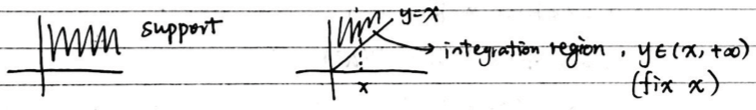
\includegraphics{0-1}
	\end{center}
	\item \textbf{Independence: } If $X,Y$ are independent, then 
	\begin{gather*}
		\textbf{Continuous: }\quad \quad f(x,y) = f_X(x)f_Y(y)\\
		\textbf{Discrete: }\quad \quad P(X=x, Y=y) = P(X=x) P(Y=y)
	\end{gather*}
	\item \textbf{Convolution: } assume $X,Y$ are independent
	\begin{gather*}
		\textbf{Discrete: }\quad \quad P_{X+Y}(a) = \sum\limits_y P_X(a-y)P_Y(y) = \sum\limits_x P_X(x)P_Y(a-x)\\
		\textbf{Continuous: }\quad \quad f_{X+Y}(a) = \int_y f_X(a-y)f_Y(y)dy = \int_y f_X(x)f_Y(a-x)dx\\
		\textbf{MGF: }\text{we can use this} \quad \quad M_{X+Y}(t) = M_X(t) M_Y(t) \longrightarrow \text{then identify dist of X+Y from mgf} 
	\end{gather*}
\end{itemize}
\subsection*{Conditional distribution}
\begin{align*}
	\textbf{Discrete} \quad \quad
	& P_{X|Y=y}(x|y) = \frac{P_{X,Y}(x,y)}{P_Y(y)} = \frac{P(X=x, Y=y)}{P(Y=y)}\\
  & \Rightarrow \sum\limits_y P_{X,Y}(x,y) = \sum\limits_y P_{X|Y=y}(x|y) \cdot P_Y(y)\\
  \textbf{Continuous} \quad \quad & f_{X|Y=y}(x|y) = \frac{f_{X,Y}(x,y)}{f_Y(y)}\\
  & \Rightarrow f_X(x) = \int_y f(x,y)dy = \int_y f_{X|Y=y}(x|y)\cdot f_Y(y)dy
\end{align*}
\subsubsection*{Conditional Expectation}
\begin{align*}
	& E[X|Y=y] = \int_x xf(x|y) dx\\
	& E[X|Y]: \text{compute } E[X|Y=y] \text{ first, replace $y$ with $Y$}
\end{align*}
\subsection*{Ordered Statistics}
Consider $X_1, X_2, \cdots, X_n \quad \quad X_{(j)}$ = j-th smallest
\begin{align*}
	F_{\max(X_i)}(t) & = P(\max X_i \leq t) = P(X_1 \leq t)\cdot P(X_2 \leq t) \cdots P(X_n \leq t)\\
	& = [F_X(t)]^n \quad \quad \quad
	\boxed{f_{\max X_i}(t) = nF(t)^{n-1} f_X(t)}\\
	 F_{\min(X_i)}(t) & = 1 - P(\min x_i \geq t) = 1-P(X_1 \geq t)\cdot P(X_2 \geq t) \cdots P(X_n \geq t)\\
	 & = 1 - [1 - F_X(t)]^n \quad \quad \quad \boxed{f_{\min X_i}(t) = n[1 - F(t)]^{n-1} f_X(t)}
\end{align*}
\textbf{General:} $j$-th order statistic
\begin{equation*}
	f_{x(j)}(t) = \binom{n}{j-1,1,n-j} F_X(t)^{j-1}\cdot f_X(t) \cdot [1-F_X(t)]^{n-j}
\end{equation*}
\subsection*{Expectation and Variance}
\begin{gather*}
	\textbf{Law of Total Expectation: } E[X] = E[E[X|Y]]\\
\textbf{Law of Total Variance: } Var(X) = E[Var(X|Y)] + Var[E(X|Y)]
\end{gather*}
\subsubsection*{Expectation}
\begin{enumerate}[label=\protect\circled{\arabic*}]
	\item linearity of expectation
	\item How to compute
	\begin{enumerate}
		\item LOTUS or definition (use density to integrate)
		\item MGF: $M^{(n)}(0) = E[X^n]$ or by recognition
		\item $E[X^2] = Var[X] + E[X]^2$
		\item Tail probability X is non-neg R.V. $(x>0)$ then $E[X] = \sum\limits_{t=0}^\infty P(X \geq t)$ \textit{or} $= \int\limits_0^\infty P(X \geq t) dt$
	\end{enumerate}
\end{enumerate}
\subsubsection*{Variance}
\begin{enumerate}[label=\protect\circled{\arabic*}]
	\item $Var(X_1 + X_2 + \cdots + X_n) = \sum\limits_{i=1}^n Var(X_i) + \sum\limits_{i \neq j} Cov(X_i, X_j)$
	\begin{center}
		if $X_i, X_j$ identical (not independent) $ = n Var(X_i) + n(n-1)Cov(X_i, X_j) \quad \quad i\neq j$
	\end{center}
	\item \textbf{Covariance: }
	\begin{align*}
		Cov(X,Y) & = E[XY] - E[X]E[Y]\\
		Cov(X,c) & = 0 \quad \quad c \textit{ is a constant}\\
		Cov(X+Y,Z) & = Cov(X,Z) + Cov(Y,Z)\\
		Cov(cX,dZ) & = cd \cdot Cov(X,Z) 
	\end{align*}
	\item \textbf{Correlation Coefficient:}
	\begin{equation*}
		\rho(X,Y) = \frac{Cov(X,Y)}{\sqrt{Var(X) Var(Y)}} = \frac{Cov(X,Y)}{\sigma_x \sigma_y}
	\end{equation*}
\end{enumerate}
\subsection*{Limit Theorems}
\subsubsection*{Markov's Inequality}
For any non-negative random variable $X$
\begin{equation*}
	P(X \geq a) \leq \frac{E(X)}{a} \tag{for \underline{any} $a > 0$}
\end{equation*}
\begin{proof}
	Let $X \geq 0$ a random variable and let $a > 0$.
	Define new random variable from $X$ as $Y_a$
	\begin{gather*}
		Y_a =
		\begin{cases}
 		0 & \text{if }	X < a\\
 		a & \text{if }	X \geq a\\
		 \end{cases}\\
		0 \leq Y_a \leq X \Longrightarrow \underbrace{E[Y_a]}_{a\cdot P(X \geq a)} \leq E[X]\\
		E[Y_a] = 0 \cdot P(Y_a < a) + a\cdot P(X \geq a)\\
		 E[Y_a] = a\cdot P(X \geq a) \leq E[X] \Longrightarrow \boxed{P(X \geq a) \leq \frac{E(X)}{a}}
	\end{gather*}
\end{proof}
\subsubsection*{Chebyshev's Inequality}
For any random variable Y with mean $\mu_y$ and variance $\sigma_y^2$
\begin{equation*}
	P(|Y - \mu)y| \geq c) \leq \frac{\sigma_y^2}{c^2} \tag{for \underline{any} $c > 0$}
\end{equation*}
\begin{proof}
	\begin{gather*}
		P(|Y - \mu_y)| \geq c) = P(\underbrace{|Y - \mu_y)|^2}_{=X} \geq c^2)\\
		P(|Y - \mu_y)|^2 \geq c^2) \leq \frac{E[|Y - \mu_y|^2]}{c^2} = \frac{\sigma_y^2}{c^2}
	\end{gather*}
\end{proof}
This is the same as
\begin{itemize}[label={--}]
	\item $P(|Y - \mu_y| \geq k \sigma_y) \leq \frac{1}{k^2}$
	\item $P(|Y - \mu_y| \leq k \sigma_y) \geq \underbrace{1- \frac{1}{k^2}}_{\text{very conservative}}$
\end{itemize}
\subsubsection*{Weak Law of Large Numbers}
If $X_1, X_2, \cdots$ are $i.i.d.$ with a mean $\mu$
\begin{equation*}
	\text{then} \qquad \mathlarger{\mathlarger{\Lim{n \rightarrow \infty}}} {\large P}\bigg( \bigg| \frac{X_1 + X_2 + \cdots + X_n}{n} - \mu \bigg| \geq \epsilon \bigg) = 0
\end{equation*}
\classheader{2018-08-30}
\section*{Survey Sampling}
We have a \underline{population of objects} under study (people, animals, places, etc.). We will consider a single numerical measurement associated to object $i: x_i$
\begin{example}
	$N = 5000, x_i=$ height of person $i$, Population size = N. We denote population measurements $\{x_1, x_2, \cdots, x_N\}$\\
	Compute population quantities:
	\begin{multicols}{2}
		\begin{itemize}
		\item population total $\tau = \sum\limits_{i=1}^N x_i$
		\item population mean $\mu = \frac{\tau}{N}= \frac{\sum\limits_{i=1}^N x_i}{N}$
	\end{itemize}
	\end{multicols}

\end{example}
\textbf{Note: } $\tau$ and $\mu$ are \underline{population parameters}, their computation depends on all the population data.
\begin{question}
	 How to estimate $\tau$ and $\mu$ based on a sample of observation from this population?
\end{question}
\underline{Classical Answer:} Choose a "random" sample of objects and associated measurements denoted $\{x_1, x_2, \cdots, x_n \}$. \emph{Note: } capital $X_i$ denote random variables.\\
Whiter "Random"? Two types of ways to sample:
\begin{multicols}{2}
	\begin{itemize}[label={--}]
	\item without replacement
	\item with replacement
\end{itemize}
\end{multicols}
\begin{claim-N}
	If $X_i$ are drawn without replacement, then the distribution of $X_1$ and $X_2$ are identical. Is this true? \textbf{In fact, \underline{\Large it is}} $\Rightarrow$ They are \textbf{\underline{\large NOT}} independent but they are identically distributed.
\end{claim-N}
\begin{center}
	P(Ace in Pos 1) = P(Ace in Pos 2) = $\frac{4}{52}$
\end{center}
\subsubsection*{Combinatorial Approach}
"well-shuffled deck" $\leftrightarrow$ all $52!$ rearrangements of the card are equally likely. How many rearrangements have ace at pos 1? \underline{$4 \cdot 51!$}
\begin{equation*}
	P(A_1) = \frac{4 \cdot 51!}{52!} = \frac{4}{52} = P(A_2) = P(A_{19}) = P(A_{36})
\end{equation*}
\begin{question}
	If $X_1$ and $X_2$ are identically distributed, then how do they differ between corresponding draws with replacement?
\end{question} 
\begin{answer}
	Independence. We can have Random Variables that are identically distributed and not independent. Note if independent, $P(A_2 |A_1) = P(A_2)$.
\end{answer}
\begin{equation*}
	\begin{split}
		\textbf{with replacement}\\
		P(A_1) = \frac{4}{52}, \quad
		P(A_2) = \frac{4}{52}\\
		P(A_2 | A_1) = \frac{4}{52}
	\end{split} \hspace{10em}
	\begin{split}
		\textbf{without replacement}\\
		P(A_1) = \frac{4}{52}, \quad
		P(A_2) = \frac{4}{52}\\
		P(A_2 | A_1) = \frac{3}{51}
	\end{split}
\end{equation*}
We can see from this that depending on sampling method, we gain or lose independence. In the finite population sampling method, we have $1, \ldots, N$ objects we care about. \\
\textbf{Loss of Independence} when choosing sampling method is important. 
\classheader{2018-09-05}
Finite Population sampling -- without $i$ without replacement. Mean/expected value and variance of $\bar{X}$\\
Suppose our population is given by $\{x_1, \ldots, x_N\} = \{1,2,2,7,8,9 \}$ where
\begin{center}
	$N = 6$, \quad $x_1 = 1$ \quad $x_2 = 2$\quad $x_3 = 2$ \quad $x_4 = 7$ \quad $x_5 = 8$\quad $x_6 = 9$
\end{center}
Could also describe it by counting.
\begin{center}
	\begin{tabular}{c|c}
		Distinct Value & frequency\\
		\hline
		$\varphi_1 = 1$ & $n_1=1$\\
		$\varphi_2 = 2$ & $n_2=2$\\
		$\varphi_3 = 7$ & $n_3=1$\\
		$\varphi_4 = 8$ & $n_4=1$\\
		$\varphi_5 = 9$ & $n_5=1$\\
	\end{tabular}
\end{center}
Possible sample of size $n=6$, where we sample \underline{without replacement}
\begin{center}
	$X_1 = 7$ \quad $X_2 = 2$ \quad $X_3 = 8$ \quad $X_4 = 9$ \quad $X_5 = 1$ \quad $X_6 = 2$ \quad
\end{center}
Sample here is the same as population as $\circled{n=N}$\\
Same thing \underline{with replacement}
\begin{center}
	$X_1 = 9$ \quad $X_2 = 9$ \quad $X_3 = 9$ \quad $X_4 = 9$ \quad $X_5 = 9$ \quad $X_6 = 9$
\end{center}
Typically $N$ is large and $n << N$\\
Recall population parameters
\begin{equation*}
	\mu = \frac{\sum\limits_{i=1}^{N} X_i}{N} \hspace{5em} \tau = N \mu = \sum\limits_{i=1}^N X_i
\end{equation*}
Next, $\sigma^2$ (population variance)
\begin{equation*}
	\sigma^2 = \frac{1}{N} \sum\limits_{i=1}^N(x_i - \mu)^2 \tag{$\sigma^2$ is pop. variance}
\end{equation*}
Alternatively, we can also express $\sigma^2$ as
\begin{gather*}
	\sigma^2 = \frac{\sum\limits_{i=1}^N(x_i - \mu)^2}{N}  = \frac{\sum\limits_{i=1}^N(x_i^2 - 2\mu x_i + \mu^2)}{N}\\
	= \frac{\sum\limits_{i=1}^N x_i^2}{N} - \frac{2\mu}{N} \underbrace{\sum\limits_{i=1}^Nx_i}_{\mu} + \frac{\cancel{N}\mu^2}{\cancel{N}}\\
	= \frac{\sum\limits_{i=1}^N x_i^2}{N} - 2\mu^2 + \mu^2\\
	= \underbrace{\bigg(\frac{1}{N} \sum\limits_{i=1}^N x_i^2 \bigg)}_{\text{2nd moment}} - \mu^2 = \mu^{(2)} - \mu^2
\end{gather*}
\textbf{Define: } $\mu^{(k)} = \frac{1}{N} \sum\limits_{i=1}^N x_i^k$
\subsection*{Sample Mean $\bar{X}$ as an estimator}
A function of the sample data for the population $\mu$.\\
\emph{Note: } If the sample is random $(X_1, \ldots, X_n \text{ are R.Vs})$, then $\bar{X}$ is \textbf{random!}\\
\underline{Questions:} 
\begin{enumerate}[label=\protect\circled{\arabic*}]
	\item How is $\bar{X}$ distributed? - in theory, if we know $\circled{1}$, then we know the answers $\circled{2}$ \& $\circled{3}$ too.
	\item What is $E[\bar{X}]$?
	\item What is $Var(\bar{X})$?
\end{enumerate}
\underline{\textit{Let's address $\circled{2}$}}\\\\
\qquad Consider $E[\underbrace{X_1}_{\text{\tiny first draw}}]$ \qquad \qquad \hspace{5em} possible values for $X_1 = \{x_1, \ldots, x_N\}$
\begin{equation*}
	P(X_1 = x_k) = \frac{1}{\binom{N}{1}} = \frac{1}{N}
\end{equation*}
\textbf{e.x.} $\{\underbrace{1}_{\tiny x_1},\underbrace{2}_{\tiny x_2},\underbrace{2}_{\tiny x_3},\underbrace{7}_{\tiny x_4},\underbrace{7}_{\tiny x_5},\underbrace{9}_{\tiny x_6} \}$ \hspace{2em} {\scriptsize gives every separate entry a unique ticket even if they are the same}
\begin{equation*}
	E[X_1] = \frac{1}{N} \sum\limits_{k=1}^N x_k = \mu = E[X_2] \tag{b/c $X_1$ \& $X_2$ are identically dist.}
\end{equation*}
In sampling \boxed{\text{without replacement}} $X_i$ \& $X_j$ are \underline{still identically} distributed, but they are \underline{not independent}.\\
In sampling \boxed{\text{with replacement}}, $X_i$ \& $X_j$ are $i.i.d.$\\
Note that whether or not $X_1, \cdots, X_n$ are independent, 
\begin{equation*}
	E\bigg[\sum\limits_{i=1}^N X_i\bigg] = \sum\limits_{i=1}^N E[X_i]
\end{equation*}
\emph{Note:} The sample mean is equal to expected population mean regardless of sampling with or without replacement.
\begin{align*}
	E[\bX] = E\bigg[\frac{1}{n} \sum\limits_{i=1}^n X_i \bigg] = & \frac{1}{n} \sum\limits_{i=1}^N E[X_i]\\
	= & \frac{n\mu}{n} = \mu 
\end{align*}
Since $E[\bX] = \mu$, we say $\bX$ is an \underline{unbiased} estimator for $\mu$. \qquad \textbf{BUT} $\underbrace{\bX}_{\text{\tiny R.V.}} \neq \overbrace{\mu}^{\text{constant}}$\\
\underline{\textit{Let's address $\circled{3}$}}

\subsubsection*{Sampling with replacement.}
Here $X_1, \cdots, X_n$ are $i.i.d.$. In general, $X_i$s are R.V. and $a_i$s are constants
\begin{equation*}
	Var\big(\sum a_i X_i\big) = \sum\limits_i \sum\limits_j a_i a_j cov(X_i, X_j) 
\end{equation*}
If $X_1, \cdots, X_N$ are independent, $\underset{i \neq j}{Cov(X_i, X_j)} = 0$! Hence
\begin{gather*}
	Var(\bX) = Var\bigg(\frac{1}{n} \sum\limits_{i=1}^n X_i \bigg) = \frac{1}{n^2} Var\bigg( \sum\limits_{i=1}^n X_i \bigg) = \frac{1}{n^2}  \sum\limits_{i=1}^n \underbrace{Var(X_i)}_{\text{a constant}}\\
	\boxed{Var(\bX) = \frac{Var(X_i)}{n}}
\end{gather*}
We need to compute $Var(X_i)$. Observe that $Var(X_i)$ are same for all: \textit{Why?} because they are identical.\\
Also notice $\frac{Var(X_i)}{n}$ decreases with $n$.\\
Observe that for all finite $n$, $Var(\bX)$ is not 0 unless $Var(X_i) = 0$!\\
\emph{Note:} $Var(X_i) = E[(X_i - E(X_i))^2] = E[(X_i - \mu^2)] = \frac{1}{N} \sum (x_i - \mu)^2 = \sigma^2$\\
\underline{So} $Var(X_i) = 0$ \textbf{iff} all $X_i \equiv \mu$
\begin{lemma}
	$bX$ is \underline{consistent} for $\mu$, i.e. $\forall \delta > 0$, the $P(|\bX - \mu| > \delta) \longrightarrow 0$ as $n\rightarrow \infty$
\end{lemma}
For this Lemma, we need to Prove Chebyshev's Inequality, which is
\begin{equation*}
	P(|Z - E(Z)| > \delta) \leq \frac{Var(Z)}{\delta^2}
\end{equation*}
Use this identity!
\begin{gather*}
	E[\bX] = \mu, \hspace{5em} Var(\bX) = \frac{\sigma^2}{n}\\
	P(|\bX - E(\bX)| > \delta) \leq \frac{Var(\bX)}{\delta^2} = \frac{\sigma^2}{n\delta^2} \rightarrow 0 \qquad \text{as } n \rightarrow \infty
\end{gather*}
\subsubsection*{Sampling without replacement}
\classheader{2018-09-10}
\subsubsection*{Sampling without replacement}
$Var(\bar{X}) =$ when sampling without replacement\\
\begin{theorem}
	Sampling from finite population without replacement
	\begin{equation*}
		Var(\bar{X}) = \frac{\sigma^2}{n} \bigg[ \underbrace{\frac{N-n}{n-1} }_{\text{FPN}} \bigg] \tag{finite population correction}
	\end{equation*}
\end{theorem}
\underline{Points to Note} - In sample without replacement,
\begin{itemize}[label={--}]
	\item If $n = N$, $Var(\bar{X}) = 0$
	\item If $n=1$, $Var(\bar{X}) = \frac{\sigma^2}{n} = \sigma^2$, same as with replacement
	\item Check: for $n > 1$, how does $\frac{N-n}{N-1}$ relate to 1? The $Var(\bar{X})$ is \underline{always} less without replacement
\end{itemize}
\begin{proof}Start\\
\begin{enumerate}[label=\protect\circled{\arabic*}]
	\item
	\begin{gather*}
		Var(\bar{X}) = Var\bigg(\frac{1}{n} \sum\limits_{i=1}^n X_i \bigg) = \frac{1}{n^2} \sum_i \sum_j Cov(X_i, X_j)\\
		\bigg( \text{When sampling with replacement, } Cov(X_i, X_j) = 0 \text{ if } i \neq j \bigg)
	\end{gather*}
	In sampling without replacement, we cannot assert that $Cov(X_i, X_j) = 0$ and we'll compute it explicitly. 
	\begin{align*}
		\text{Recall} \qquad Cov(X_i, X_j) & = E[X_i X_j] - \underbrace{E[X_i] E[X_j]}_{\mu^2}\\
		\mu^2 \leftarrow \text{as identical but not independent} \qquad & = E[X_i X_j] - \mu^2
	\end{align*}
	\item To calculate $E[X_i X_j]$, let us list distinct values in population
	\begin{example}
	$\{\underbrace{5}_{x_1}, \underbrace{5}_{x_2}, \underbrace{8}_{x_3}, \underbrace{11}_{x_4}, \underbrace{8}_{x_5}, \underbrace{17}_{x_6}, \underbrace{9}_{x_7}\}$ Let $n_l$ = $\#$ of times $\zeta_l$ appears in population.
	\begin{center}
		\begin{tabular}{c|c}
		Distinct Value & frequency\\
		\hline
		$\zeta_1 = 5$ & $n_1=2$\\
		$\zeta_2 = 8$ & $n_2=2$\\
		$\zeta_3 = 11$ & $n_3=1$\\
		$\zeta_4 = 17$ & $n_4=1$\\
		$\zeta_5 = 9$ & $n_5=1$\\
	\end{tabular}
	\end{center}
	\end{example}
	\begin{gather*}
		P[X_i = 5] = \frac{2}{7} = \frac{n_1}{N} \tag{i draws identical}\\
		\Rightarrow P[X_i = \zeta_l] = \frac{n_l}{N}\\
		n_1 + n_2 + \ldots + n_m = \sum_{j=1}^m n_j = N\\
		E[X_i X_j] = \sum_{k=1}^m \sum_{l=1}^m \zeta_k \zeta_l \underbrace{P[X_i = \zeta_k, X_j = \zeta_l]}_{\text{?}}
	\end{gather*}
	\begin{gather*}
		P[X_i = \zeta_k, X_j = \zeta_l] = \underbrace{P[X_j = \zeta_l| X_i = \zeta_k]}_{\circled{3}} \cdot \underbrace{P[X_i = \zeta_k]}_{ = \frac{n_k}{N}}
	\end{gather*}
	\item Cases for Conditional probability
	\begin{gather*}
		P[X_j = \zeta_l| X_i = \zeta_k] \stackrel{cases}{=} \begin{cases}
			\frac{n_l}{N_1} & l \neq k \rightarrow \text{numbers are diff.}\\
			\frac{n_l - 1}{N - 1} & l = k \rightarrow \text{numbers are same}
		\end{cases}
	\end{gather*}
	\item So we have
	\begin{gather*}
		E[X_i X_j] = \sum_{k=1}^m \sum_{l=1}^m \zeta_k \zeta_l P[X_i = \zeta_k, X_j = \zeta_l]\\
		E[X_i X_j] = \sum_{k=1}^m \sum_{l=1}^m \tikzmark{a}{\zeta_k} \zeta_l P[X_j = \zeta_l| X_i = \zeta_k] \cdot \tikzmark{b}{P[X_i = \zeta_k]}
		\begin{tikzpicture}[overlay, remember picture]
		\draw[-, red](a) to [out=-40,in=200](b);
		\draw[decorate] (a) to [out=-40,in=200] (b);
		\end{tikzpicture}\\
		= \sum_k \zeta_k P[X_i = \zeta_k] \zeta_k \bigg( \sum_l \zeta_l P[X_j = \zeta_l| X_i = \zeta_k] \bigg)\\
		= \sum_k \zeta_k P[X_i = \zeta_k] \zeta_k \bigg( \sum_{l\neq k} \zeta_l P[X_j = \zeta_l| X_i = \zeta_k] + \zeta_k P[X_j = \zeta_k | X_i = \zeta_k] \bigg)\\
		= \sum_k \zeta_k P[X_i = \zeta_k] \zeta_k \bigg( \underbrace{\sum_{l\neq k} \zeta_l \frac{n_l}{N-1}}_{\circled{5}} + \zeta_k \frac{n_k - 1}{N - 1} \bigg)
	\end{gather*}
	\item When $l \neq k$ and we want to remove all $l$ terms
	\begin{gather*}
		\sum_{l\neq k} \zeta_l \frac{n_l}{N-1} = \frac{1}{N-1} \sum_{l \neq k} \zeta_l n_l\\
		\bigg(\sum_l \zeta_l n_l = \tau = n\mu \bigg) \quad \text{population total}\\
		 = \frac{1}{N-1} (\tau - \zeta_k n_k)
	\end{gather*}
	\item \underline{Now Back}
	\begin{align*}
		E[X_i X_j] & = \sum_k \zeta_k \frac{n_k}{N} \bigg( \frac{1}{N-1} (\tau - \zeta_k n_k) + \zeta_k \frac{n_k - 1}{N-1} \bigg)\\
		& = \frac{1}{N(N-1)} \sum_k \zeta_k n_k \big[ (\tau - \cancel{\zeta_k n_k}) + \cancel{\zeta_k n_k} - \zeta_k \big]\\
		& = \frac{1}{N(N-1)} \sum_k \zeta_k n_k \big[\tau - \zeta_k \big]\\
		& = \frac{1}{N(N-1)} \bigg( \sum_k \zeta_k n_k \tau - \sum_k \zeta_k^2 n_k \bigg)\\
		& = \frac{1}{N(N-1)} \bigg[ \tau^2 - \sum_k \zeta_k^2 n_k \bigg]
	\end{align*}
	\item What is $\sum\limits_k (\zeta_k)^2 \frac{n_k}{N}$? Second moment $E[X_i^2]$ \qquad $E[X_i^2] = \sigma^2 + \mu^2$
	\begin{gather*}
		E[X_i^2] = \sigma^2 + \mu^2 \qquad \frac{\tau^2}{N} = N\mu^2 as \mu = \frac{\tau}{N}\\
		E[X_i X_j] \Longrightarrow \frac{1}{N-1} \bigg[N\mu^2 - (\sigma^2 + \mu^2) \bigg]\\
		 = \frac{1}{N-1}[(N-1)\mu^2 - \sigma^2] = \mu^2 - \frac{\sigma^2}{N-1}
	\end{gather*}
	\begin{align*}
		\text{So} \quad Cov(X_i, X_j) & = \mu^2 - \frac{\sigma^2}{N-1} - \mu^2\\
		& = -\frac{\sigma^2}{N-1} \tag{Cov $< 0$}\\
		\text{So} \quad Cov(X_i, X_j) & = Var(X_i) = \sigma^2\\
	\end{align*}
	\item Putting it all together
	\begin{align*}
		Var(\bX) & = \frac{1}{n^2} \bigg(\sum_{i\neq j} Cov(X_i, X_j) + \sum_{i=1}^n Var(X_i) \bigg)\\
		& = \frac{1}{n^2} \bigg(\sum_{i\neq j} -\frac{\sigma^2}{N-1} + n\sigma^2 \bigg)\\
		& = \frac{1}{n^2} \bigg(\frac{-n(n-1)\sigma^2}{N-1} + \frac{\sigma^2}{n} \bigg)\\
		& = \frac{\sigma^2}{n} \bigg(1 - \frac{n-1}{N-1} \bigg)\\
		& \boxed{ = \frac{\sigma^2}{n} \bigg(\frac{N-n}{N-1} \bigg)}
	\end{align*}
\end{enumerate}
\end{proof}
 
\classheader{2018-09-12}
\begin{itemize}
	\item Binary data- special case.
	\item Approximate distance of $\bX$ when $n$ is large but $n << N$
	\item Estimating population Variance
	\item Bivariate data
\end{itemize}
Recall that population is \underline{dichotomous} or \underline{binary} then $x_i = \begin{cases}
	1\\0
\end{cases}$\\
Moreover if we consider $x_i = 1$ as a "success" and $x_i = 0$ as a "failure", then
\begin{equation*}
	\mu = \frac{\sum_{i=1}^N X_i}{N} = \frac{\text{\# of successess in population}}{\text{population size}} = p \tag{$\text{pop}^n$ proportion of success}
\end{equation*}
\begin{gather*}
	\text{Now,} \quad \sigma^2 = \underbrace{\frac{\sum_{i=1}^N X_i}{N}}_{\mu} - \mu^2 = p - p^2 = p(1-p) = pq\\ \begin{align*}
				\mu \text{ as } & 1 \Rightarrow 1^2 = 1
				& 0 \Rightarrow 0^2 = 0
	\end{align*}
\end{gather*}
Recall that if $Y \sim \text{Bernoulli}(p)$, $Y_i = \begin{cases}
	1 & \text{w/ prob } p\\0 & \text{w/ prob } 1-p
\end{cases}$\\
\begin{gather*}
	E[Y] = p\\
	Var(Y) = p(1-p)
\end{gather*}
Last few weeks involved an analysis of $\bX$, $E(\bX)$, $Var(\bX)$. Could also ask: How is $\bX$ distributed if $n$ is large.
\subsection*{Confidence Intervals - Sampling W.R.}
If sampling \textbf{with replacement}, where $X_1, \ldots, X_n$ denotes sample, we know $X_i$'s are $i.i.d.$ Hence when $n$ is large, by CLT $\bX$ has an approximately normal distribution.
\begin{equation*}
	P \bigg(\frac{\bX - \mu}{\sigma/ \sqrt{n}} \leq x \bigg) \longrightarrow \Phi(x) \qquad \text{as } n \rightarrow \infty
\end{equation*}
When sampling with replacement, we can use this to obtain confidence intervals for $\mu$: Let $\alpha \in (0,1)$ be given.
\begin{center}
	Let $Z_\alpha \in \mathbb{R}$ such that $P(Z > Z_\alpha) = \alpha$ where $Z \sim N(0,1)$
\end{center}
By the Central Limit Theorem, for $n$ large (sampling w/replacement)
\begin{gather*}
	= P \bigg( - Z_{\alpha / 2} \leq \frac{\bX - \mu}{\sigma/ \sqrt{n}} \leq Z_{\alpha / 2} \bigg)\\
	= P \bigg(\underbrace{\bX - Z_{\alpha / 2}\cdot \frac{\sigma}{\sqrt{n}}}_{\text{Random}} \leq \mu \leq \underbrace{\bX + Z_{\alpha / 2}\cdot \frac{\sigma}{\sqrt{n}}}_{\text{Random}} \bigg)\\
	Var(\bX) = 0 \qquad \text{Never happens}
\end{gather*}
\begin{center}
	\begin{tikzpicture}[scale=0.6]
    		\draw[very thick,-] (-6,0) -- (6.2,0);
		    \draw[very thick,-] (0,-1) -- (0,6.2) node[above] {$\mu$};

			\draw[<->] (-4,5) -- (1,5) node[right] {sample 1};			
			\draw[<->] (-2,4) -- (5,4) node[right] {sample 2};
			\draw[<->] (1,3) -- (6,3) node[right] {sample 3};
		    \draw[<->] (-6,2) -- (-3,2) node[right] {sample 4};
		    \draw[<->] (-1,1) -- (4,1) node[right] {sample 5};
			\end{tikzpicture}
\end{center}
In repeated sampling, approx $(1 - \alpha)$ of intervals contain $\mu$, and ($\alpha$) frac will not.
\begin{center}
	We say $\boxed{\bX - Z_{\alpha / 2}\cdot \frac{\sigma}{\sqrt{n}}}$ is $100(1-\alpha)$\% 2-sided confidence interval for $\mu$
\end{center}
\textbf{Problem: }This interval involved $\sigma$ which is unknown. Observe that if $n$ is large, then $\frac{\bX - \mu}{\sigma/ \sqrt{n}}$ is still approx $N(0,1)$ in distribution where (no population parameters)
\begin{gather*}
	\tcbhighmath[drop fuzzy shadow]{s^2 = \frac{1}{n-1} \sum(X_i - \bX)} \tag{sample variance}
\end{gather*}
So we obtain 
\begin{gather*}
	\tcbhighmath[drop fuzzy shadow]{\bX \pm Z_{\frac{\alpha}{2}} \frac{s}{\sqrt{n}}} \qquad \text{as a $100(1-\alpha)$ CI for $\mu$}
\end{gather*}
\redhline\\\\
In the dichotomous case, 
\begin{gather*}
	\bX = \frac{\text{\# of the succession sample}}{\text{sample size}} = \hat{p}\\
	100(1-\alpha)\% \text{ CI for } \qquad p: \hat{p} \pm Z_{\frac{\alpha}{2}} \sqrt{\frac{\hat{p}(1-\hat{p})}{n}}
\end{gather*}
\subsection*{Confidence Intervals - Sampling W.o.R.}
Recall now what happens when sampling \textbf{without replacement}
\begin{center}
	Here, $X_1, X_2, \ldots, X_n$ remain identically distributed, but not independent
\end{center}
We surmised, that if $n << N$, $X_i \& X_j$ have an \textit{"approximate independence"}
\begin{example-N}
	Let population consist of 1000 elements. In this case:
	\begin{gather*}
		\text{blue } - \circled{1} - 200, \qquad \text{red } - \circled{2} - 300, \qquad \text{green } - \circled{1} - 500\\
		\begin{rcases}
		P(X_1 = \circled{3}) = \frac{1}{2}\\
		P(X_2 = \circled{3} | X_1 = \circled{3}) = \frac{499}{999}
		\end{rcases} \text{not independent, but have approximate independence.}
	\end{gather*}
\end{example-N}
In short, $n << N$, each successive draw does not alter probabilities that much, precisely b/c removal is only of a sample \# of population elements.\\
So if $n << N$, then even in sampling W.O.R, $X_i$'s retain an approximate independence. Further if $n$ is "large" and small relative to $N$, (note delicate point!) then $\bX$ will still have an approx Normal distribution.
\begin{gather*}
	\mathlarger{\frac{\bX - \mu}{\sqrt{\frac{\sigma^2}{n} \big(\frac{N-n}{N-1} \big)}}} \sim N(0,1)
\end{gather*}
Observe $\sigma^2$ us still unknown. We'd like to consider estimators for $\sigma^2$
\subsection*{Estimator for variance W.o.R}
\begin{gather*}
	\hat{\sigma}^2 = \frac{1}{n} \sum_{i = 1}^n (X_i - \bX)^2\\
	s^2 = \frac{1}{n-1} \sum_{i = 1}^n (X_i - \bX)^2
\end{gather*}
Try to understand $E[\hat{\sigma}^2]$
\begin{gather*}
	\hat{\sigma}^2 = \frac{1}{n} \sum_{i = 1}^n (x_1^2 -2x_i \bX + \bX^2)\\
	\hat{\sigma}^2 = \frac{\sum\limits_{i=1}^n x_i^2}{n} - 2\bX \bX	 + \bX^2 = \frac{\sum\limits_{i=1}^n x_i^2}{n} - \bX^2\\
	E[\hat{\sigma}^2] = E \bigg[\frac{\sum\limits_{i=1}^n x_i^2}{n}\bigg] - E[\bX^2] \qquad \text{can't get $E[\bX^2]$ from $Var(\bX)$}\\
	Var(\bX) = E[\bX^2] - (E[\bX^2])^2\\
	\underbrace{Var(\bX)}_{\text{computed}} + \mu^2 = E[\bX^2]\\
	E \bigg[\frac{1}{n} \sum_{i=1}^n \bigg] = \frac{1}{n} \sum_{i=1}^n E[X_i^2] = \sigma^2 + \mu^2\\
	\text{Combining, we get: }\\
	E[\hat{\sigma}^2] = \sigma^2 + \mu^2 - (Var(\bX) + \mu^2)\\
	= \sigma^2 - \bigg[\frac{\sigma^2}{n} \bigg(\frac{N-n}{N-1} \bigg) \bigg]
\end{gather*}
The estimator is biased, but
\begin{gather*}
	= \sigma^2 \bigg(\underbrace{1 - \frac{N-n}{(n)(N-1)}}_{\text{constant, }c} \bigg)\\
	= C \sigma^2
\end{gather*}
and thus $\frac{\hat{\sigma}^2}{C}$ is an unbiased estimator.

\classheader{2018-09-17}
\begin{itemize}
	\item Approximation methods / Delta-methods
	\item Bivariate populations
	\item Ratio estimations
\end{itemize}
We calculated $E\underbrace{[\hat{\sigma}^2]}_{C\sigma^2}$ where $\hat{\sigma}^2 = \frac{1}{n} \sum\limits_{i=1}^n (X_i - \bX)^2$ and you can use our computations to generate an unbiased estimator for population variance $\sigma^2$. Can also use his to calculate $E[s^2]$, where $s^2 = \frac{1}{n-1} \sum\limits_{i=1}^n (X_i - \bX)^2$
\subsection*{Bias-Variance Tradeoff}
\begin{enumerate}[label=\protect\circled{\arabic*}]
	\item Unbiased estimators are useful: if $T$ is an unbiased estimator for $\theta$ then $E[T] = \theta$.
	\item However, if we wish to evaluate two estimatorsL- one biased and other unbiased, we may not universally want to choose the unbiased one always, we need to consider \boxed{variance}.
\end{enumerate}
\underline{Why?} Suppose that T is an estimator for $\theta$.\\
\textbf{The Mean Squared Error (MSE):}
\begin{equation*}
	MSE = E[(T - \theta)^2] \xrightarrow{\text{exercised}} \underbrace{Var(T)}_{\text{Variance}} + \underbrace{(E(T) - \theta)^2}_{\text{Bias}}
\end{equation*}
\begin{center}
\begin{tikzpicture}
\begin{axis}[
  no markers, domain=-2:2, samples=100,
  axis lines*=center, xlabel=$x$, ylabel=$y$,
  every axis y label/.style={at=(current axis.above origin),anchor=south},
  every axis x label/.style={at=(current axis.right of origin),anchor=west},
  height=5cm, width=12cm,
  xtick={4,6.5}, ytick=\empty,
  enlargelimits=false, clip=false, axis on top,
  grid = major
  ]
	%\draw[-] (0,0) -- (0,0.6 ) node[left] {$y$};
  \addplot [very thick,red!50!black] {gauss(0,1)};
  \addplot [very thick,cyan!50!black] {gauss(0.5,0.5)};
  \end{axis}
\end{tikzpicture}
\end{center}
We can see from the above plots that the red graph has an estimator $\theta$ closer to $\mu$, but has a higher variance. However, estimator B has an unbiased estimator, but has a smaller variance. Depends on sampling analysis.
\subsection*{Bivariate population sampling}
Suppose we have a population of $N$ objects. On each object we have a \underline{pair} of measurements: $(x_i, y_i)$\\
\emph{Note: } When sampling from this population if object $i$ is in sample, then both measurements in pair $(x_i, y_i)$ are retained. In particular $(x_i, y_i)$ appears exactly once in the population, and sample w/o repl, then you cannot retrieve measurement $i$ later.\\
\subsubsection*{Parameters}
\begin{multicols}{3}
	\begin{gather*}
	\sigma_Y^2 = \frac{1}{N} \sum_{i=1}^N (y_i - \mu_Y)^2\\
	\mu_X = \frac{1}{N} \sum_{i=1}^N X_i\\ 
	\mu_Y = \frac{1}{N} \sum_{i=1}^N Y_i\\
	\tau_X = N\mu_X\\ \tau_Y = N\mu_Y\\
	\sigma_X^2 = \frac{1}{N} \sum_{i=1}^N (x_i - \mu_X)^2
	\end{gather*}
\end{multicols}
\subsubsection*{Covariance}
\begin{gather*}
	\sigma_{XY}^2 = \frac{1}{N} \sum_{i=1}^N (x_i - \mu_X)(y_i - \mu_Y)
\end{gather*}
Suppose $\mu_X \neq 0$ \hspace{5em} Define $r = \frac{\mu_X}{\mu_Y}$ \hspace{5em} What is a reasonable estimator $r$?\\
Could consider $R = \frac{\bX}{\bar{Y}}$\\
\redhline\\\\
Now Suppose that $\mu_X$. were known. Consider $\mu_X \cdot R = \frac{\mu_X}{\bX} \bar{Y}$.\\ Plausible estimator for $\mu_Y$. But why? we already have $\bar{Y}$, an unbiased estimator for $\mu_Y$. We will see that $\mu_X \cdot R$, the so called \textbf{ratio estimate}, is
\begin{enumerate}[label=\protect\circled{\arabic*}]
	\item a biased estimate
	\item can contribute in reduction in variance relative to $\bar{Y}$
\end{enumerate}
So we will need to understand $E[R], Var(R)$ \& approximations of $E[R]$ \& $Var(R)$
\subsection*{Approximation Methods}
Let $X$ be a random variable with mean = $\mu_X$ and variance = $\sigma_X^2$. Let $Z = g(X)$, where $g: \mathbb{R} \rightarrow \mathbb{R}$, $g$ a deterministic function of $x$.\\
\textbf{Question:} How to compute $E[Z]$?\\
\emph{Answer: } If density of $X$ is known, (call this $f_X$), then 
\begin{gather*}
	E(Z) = \int_\mathbb{R} g(X) f_X(x)dx \hspace{2em} \text{involves an integral}
\end{gather*}
Cumbersome even if $f_X$ is known; closed form solution to integral exists; not possible to get exact value even if $f_X$ known, but no closed form solution; not even possible to write integral if $f_X$ unknown. If $g$ is linear, then it is OK e.g. $E[g(X)] = E[aX + b] = a\mu_X + b$
\subsubsection*{Taylor Expansions}
Taylor expansion of $g$ about $\mu_X$ (Why? Think Chebyshev!)
\begin{gather*}
	g(x) \approx g(\mu_X) + g'(\mu_X) (x - \mu_X) + \frac{g''(x)(x - \mu_X)^2}{2!} + \cdots + \text{\small higher order terms}\\
	\tcbhighmath[drop fuzzy shadow]{g(X) \approx g(\mu_X) + g'(\mu_X) (X - \mu_X) + \frac{g''(X)(X - \mu_X)^2}{2!}}
\end{gather*}
\begin{gather*}
	E[Z] \approx E[g(\mu_X)] + E[g'(\mu_X)(X - \mu_X)] + E\bigg[\frac{g''(\mu_X)}{2!} (X - \mu_X)^2 \bigg]\\
	\approx g(\mu_X) + g'(\mu_X) \cancelto{0}{E[(X - \mu_X)]} + \frac{g''(\mu_X)}{2!} E[ (X - \mu_X)^2]\\
	\tcbhighmath[drop fuzzy shadow]{E[Z] \approx g(\mu_X) + \frac{g''(\mu_X)}{2!} \sigma^2_X}
\end{gather*}
But $R = \frac{\bar{Y}}{\bX}$, a function of \underline{two variables}!
\begin{center}
	$\text{Consider} \qquad g(x,y) : \mathbb{R}^2 \rightarrow \mathbb{R}$\\
	Taylor expand $g$ about $(\mu_x, \mu_y)$
\end{center}
\begin{enumerate}[label=\protect\circled{\arabic*}]
	\item \underline{Linear Approximation}
	\begin{gather*}
		g(x,y) \approx g(\mu_x, \mu_y) + \dfrac{\partial g}{\partial x}(\mu_x, \mu_y) \cdot (x - \mu_x) + \dfrac{\partial g}{\partial y}(\mu_x, \mu_y) \cdot (y - \mu_y)
	\end{gather*}
	\item \underline{Second order approximation}
	\begin{gather*}
		g(x,y) \approx g(\mu_x, \mu_y) + \dfrac{\partial g}{\partial x}(\mu_x, \mu_y) \cdot (x - \mu_x) + \dfrac{\partial g}{\partial y}(\mu_x, \mu_y) \cdot (y - \mu_y)\\
		+ \frac{1}{2} \dfrac{\partial^2 g}{\partial x^2}(\mu_x, \mu_y) \cdot (x - \mu_x)^2 + \frac{1}{2} \dfrac{\partial^2 g}{\partial y^2}(\mu_x, \mu_y) \cdot (y - \mu_y)^2 + \dfrac{\partial g}{\partial x \partial y}(\mu_x, \mu_y) \cdot (x - \mu_x) (y - \mu_y) 
	\end{gather*}
\end{enumerate}
\textbf{Evaluating $E[g(X,Y)]$}
\begin{gather*}
	E[g(X,Y)] \approx g(\mu_x, \mu_y) + \dfrac{\partial g}{\partial x}(\mu_x, \mu_y) \cdot \cancelto{0}{E[(x - \mu_x)]} + \dfrac{\partial g}{\partial y}(\mu_x, \mu_y) \cdot \cancelto{0}{E[(y - \mu_y)]}\\
		+ \frac{1}{2} \dfrac{\partial^2 g}{\partial x^2}(\mu_x, \mu_y) \cdot E[(x - \mu_x)^2] + \frac{1}{2} \dfrac{\partial^2 g}{\partial y^2}(\mu_x, \mu_y) \cdot E[(y - \mu_y)^2] + \dfrac{\partial g}{\partial x \partial y}(\mu_x, \mu_y) \cdot E[(x - \mu_x) (y - \mu_y)]
\end{gather*}
When the dust settles,
\begin{gather*}
	\tcbhighmath[drop fuzzy shadow]{E[g(X,Y)] \approx g(\mu_x, \mu_y) + \frac{1}{2} \dfrac{\partial^2 g}{\partial x^2}(\mu_x, \mu_y) \cdot \sigma_X^2 + + \frac{1}{2} \dfrac{\partial^2 g}{\partial y^2}(\mu_x, \mu_y) \cdot \sigma_Y^2 + \dfrac{\partial g}{\partial x \partial y}(\mu_x, \mu_y) \cdot Cov(X,Y)}
\end{gather*}
\classheader{2018-09-19}
\begin{itemize}
	\item Approximation methods, $\Delta$-methods
	\item Ratio estimations
	\item Parametric Estimation
\end{itemize}
Let $X$ be a r.v. mean $\mu_X$ and variance $\sigma_X^2$. Let $g$ be a deterministic function $g: \mathbb{R} \rightarrow \mathbb{R}$. \\
Let $Z = g(X)$ \qquad How to approximate $E[g(X)] = g(Z)$? We could do
\begin{equation*}
	E[Z] \approx g(\mu_X) + \frac{1}{2} g''(\mu_X) \cdot Var(X)
\end{equation*}
Whether or not this approximation is accurate depends on contribution to higher order terms. \\
If $Z = g(X,Y)$, then $E[Z]$ is 
\begin{equation*}
	E[Z] \approx g(\mu_x, \mu_y) + \frac{1}{2} \dfrac{\partial^2 g}{\partial x^2}(\mu_x, \mu_y) \cdot \sigma_X^2 + + \frac{1}{2} \dfrac{\partial^2 g}{\partial y^2}(\mu_x, \mu_y) \cdot \sigma_Y^2 + \dfrac{\partial g}{\partial x \partial y}(\mu_x, \mu_y) \cdot \sigma_{XY}
\end{equation*}
\textbf{Goal:} Understand $E[R]$, $Var(R)$ where $R = \frac{\bar{Y}}{\bar{X}}$ and we are sampling W.o.R from a finite bivariate population\\
\redhline\\\\
Let's consider what happens when $g(X,Y) = \frac{Y}{X}$
\begin{gather*}
	\dfrac{\partial g}{\partial x} = \frac{-y}{x^2} \rightarrow \dfrac{\partial^2 g}{\partial x^2} = \frac{2y}{x^3} \qquad 
	\dfrac{\partial g}{\partial y} = \frac{1}{x} \rightarrow \dfrac{\partial^2 g}{\partial y^2} = 0 \qquad \dfrac{\partial^2 g}{\partial x \partial y} = -\frac{1}{x^2}
\end{gather*}
Here we will look at $g(\bX,\bar{Y}) = \frac{\bX}{\bar{Y}}$ \qquad $E[\bX] = \mu_x$ and $E[\bar{Y}] = \mu_y$
\begin{gather*}
	E[g(\bX,\bar{Y})] = E\bigg[\frac{\bX}{\bar{Y}}\bigg] \approx \frac{\mu_y}{\mu_x} + \frac{1}{2}\bigg(\frac{2 \mu_y}{(\mu_x)^3} \bigg) \sigma_{\bX}^2 + 0 - \frac{1}{\mu_x^2} \sigma_{\bX \bar{Y}}
\end{gather*}
Do we think $\mu_x R$ is unbiased for $\mu_y$ \quad \textbf{Answer: } \underline{No}, it is not unbiased b/c look at approximation
\subsubsection*{What about variance?}
Let's return for a minute on general setting for approximations of moments of functions of random variables. Again $g(X,Y) = Z$\\\\
Let's write 1st order Taylor expansion for $Z$
\begin{gather*}
	Z \approx g(\mu_x, \mu_y) + \dfrac{\partial g}{\partial x}(\mu_x, \mu_y) \cdot (x - \mu_x) + \dfrac{\partial g}{\partial y}(\mu_x, \mu_y) \cdot (y - \mu_y)
\end{gather*}
So we find 
\begin{gather*}
	Z \approx a + b(X - \mu_X) + c(Y - \mu_Y)\\
	Var(Z) \approx b^2Var(X) + c^2 Var(Y) + 2bcCov(X,Y)\\
	\approx \bigg[\underbrace{\dfrac{\partial g}{\partial x}}_{\text{b}} \bigg]^2 \sigma_X^2 + \bigg[\underbrace{\dfrac{\partial g}{\partial y}}_{\text{c}} \bigg]^2 \sigma_Y^2 + 2 \bigg[\underbrace{\dfrac{\partial g}{\partial x}}_{\text{b}} \bigg] \bigg[\underbrace{\dfrac{\partial g}{\partial y}}_{\text{c}} \bigg] \sigma_{XY}
\end{gather*}
We don't go further than linear as higher variance requires higher order moments e.g. $E[x^4] \leftarrow$ they don't matter.
\begin{gather*}
	Var(R) \approx \bigg[\dfrac{-\mu_y}{\mu_x^2} \bigg]^2 \sigma_{\bX}^2 + \bigg[ \frac{1}{\mu_x} \bigg]^2 \sigma_{\bar{Y}}^2 + 2 \bigg[\dfrac{-\mu_y}{\mu_x^2} \bigg] \bigg[\frac{1}{\mu_x} \bigg] \sigma_{\bX \bar{Y}}
\end{gather*}
Recall
\begin{gather*}
	\sigma_{\bX}^2 = \frac{\sigma_x}{n} \bigg[\frac{N-n}{N-1} \bigg] \qquad \sigma_{\bar{Y}}^2 = \frac{\sigma_y}{n} \bigg[\frac{N-n}{N-1} \bigg]\\
	\sigma_{\bX \bar{Y}} = \circled{?} \quad \frac{\sigma_{xy}}{n} \bigg[\frac{N-n}{N-1} \bigg]
\end{gather*}
Recall
\begin{gather*}
	\sigma_{XY} = \frac{1}{N} \sum_{i=1}^N (x_i - \mu_x)(y_i - \mu_y)\\
	\rho = \frac{\sigma_{xy}}{\sigma_x \sigma_y}
\end{gather*}
\classheader{2018-09-24}
\begin{itemize}
	\item Properties of estimation
	\item Method of moments
	\item Maximum Likelihood
	\item Properties of estimators
\end{itemize}

\classheader{2018-09-26}
\section*{Maximum Likelihood Estimation}
\classheader{2018-10-01}
\begin{itemize}
	\item MLEs - normal, gamma, uniform
	\item Modes of convergence
	\item Slutsky's Theorem
	\item Asymptotic properties of MLEs
\end{itemize}
\subsection*{MLEs - Normal Distribution}
Let $X_i, 1 \leq i \leq n$ be i.i.d. $\mathcal{N}(\mu, \sigma^2)$ The \underline{likelihood}
\begin{align*}
	f(x_1, \leq, x_n | \mu, \sigma^2) & = \prod_{i=1}^n f(x_i | \mu, \sigma^2)\\
	& = \prod_{i=1}^n \bigg[ \frac{1}{\sigma \sqrt{2\pi}} \exp \bigg( \frac{-(x_i - \mu)^2}{2\sigma^2} \bigg) \bigg]\\
	& = \bigg( \frac{1}{\sigma \sqrt{2\pi}} \bigg)^n \exp \bigg(\frac{-1}{2\sigma^2}  \sum_{i=1}^n (x_i - \mu)^2\bigg)\\
	\underline{\text{The log-likelihood:}} \qquad & = -n \log (\sigma \sqrt{2\pi}) - \frac{1}{2\sigma^2} \sum_{i=1}^n (x_i - \mu)^2
\end{align*}
Maximize this w.r.t. $\mu, \sigma$. Here log-likelihood depends smoothly on parameters $\rightarrow$ can consider critical points as 1st step in maximization.
\begin{gather*}
	\frac{\partial l}{\partial \mu} = \frac{2}{2\sigma^2} \sum_{i=1}^n (x_i - \mu) = 0 \Longrightarrow n\mu = \sum_{i=1}^n x_i \Longrightarrow \boxed{\hat{\mu}_{\text{MLE}} = \bX}\\
	\frac{\partial l}{\partial \sigma} = \frac{-n \cancel{\sqrt{2\pi}}}{\sigma \cancel{\sqrt{2\pi}}} - \frac{-1}{\sigma^3} \sum_{i=1}^n (x_i - \mu)^2 = 0 \Longrightarrow \frac{n}{\sigma} = \frac{1}{\sigma^3} \sum_{i=1}^n (x_i - \mu)^2 \Longrightarrow \boxed{\hat{\sigma}_{\text{MLE}}^2 = \frac{1}{n} \sum_{i=1}^n (x_i - \mu)^2}
\end{gather*}
Need to make sure two partial derivatives vanish simultaneously
\begin{gather*}
	\mu = \bX\\
	\sigma^2 = \frac{1}{n} \sum_{i=1}^n (X_i - \mu)^2 \Longrightarrow \boxed{\hat{\sigma}_{\text{MLE}} = \sqrt{\frac{1}{n} \sum_{i=1}^n (X_i - \bX)^2}}
\end{gather*}
Capital $X_i$'s because want a function of the random variables in our sample. $E[\bX] = \mu$. So $\hat{\mu}$ MLE is \underline{unbiased}. Var($\hat{\mu}_{\text{MLE}}$) = $\frac{\sigma^2}{n}$\\\\
\textbf{Question:} Is $E[\hat{\sigma}_{\text{MLE}}] = \sigma$?
\begin{equation*}
	\text{Next, } \quad \hat{\mu}_{\text{MLE}} = \bX = \frac{1}{n} \sum_{i=1}^n X_i \sim \mathcal{N}\bigg(\mu, \frac{\sigma^2}{n} \bigg)
\end{equation*}
\subsection*{Support}
Given a density function $f(x|\theta)$, we define the \underline{support} of $f$ to be
\begin{equation*}
	\supp f = \{x : f(x|\theta) > 0 \}
\end{equation*}
Suppose $\Theta$ is the space (in $\mathbb{R}, \mathbb{R}^d$) to which $\theta$ belongs:
\begin{center}
	If $X_i$'s are i.i.d.. Bernoulli($p$), then $\Theta = (0,1),  \quad \supp f = \{0,1 \}$\\
	If $X_i$'s are i.i.d.. $\mathcal{N}(\mu, \sigma^2)$, then $\Theta = \{(a,b) : a \in \mathbb{R}, b > 0  \}, \quad \supp f = \mathbb{R}$\\
\end{center}
We say that the \underline{$\supp f$ is independent} of $\theta$ if
\begin{equation*}
	\{x : f(x | \theta) > 0 \} \quad \text{is the same set for all $\theta \in \Theta$}
\end{equation*}
\subsection*{MLEs - Uniform Distribution}
Now let $X_i$ be i.i.d. Unif$[0,\theta]$ \qquad $\theta > 0$ \qquad Here $\supp f$ is not independent of $\theta$.
\begin{equation*}
	\supp f = \{x: f(x | \theta) > 0 \} \qquad f(x|\theta) \begin{cases}
		0 & x < 0\\
		\frac{1}{\theta} & 0 \leq x \leq \theta\\
		0 & x >> \theta
	\end{cases}
\end{equation*}
\underline{Joint Likelihood}
\begin{gather*}
f(x_1, x_2, \ldots, x_n | \theta) = \underbrace{\frac{1}{\theta} \cdot \frac{1}{\theta} \cdots \frac{1}{\theta}}_{\text{n times}} = \bigg( \frac{1}{\theta} \bigg)^n\\
\text{with indicator} \qquad f(x_1, x_2, \ldots, x_n | \theta) = \bigg( \frac{1}{\theta} \bigg)^n \bigg( I_{[0, \theta]}(x_1) \cdot I_{[0, \theta]}(x_2) \cdots I_{[0, \theta]}(x_n) \bigg)\\
= \bigg( \frac{1}{\theta} \bigg)^n I_{\min (x_i) \geq 0, \text{ } \max (x_i) \leq \theta}
\end{gather*}
\textbf{Note: } $\big( \frac{1}{\theta}\big)^n $ is decreasing in $\theta$
\begin{itemize}
	\item So want to choose $\theta$ as small as possible
	\item So note lower bound on $\theta$ in terms of $x_i$'s if likelihood is to remain positive.
\end{itemize}
\begin{equation*}
	\boxed{\hat{\theta}_{\text{MLE}} = \underset{i \in \{1, \ldots, n\}}{\max} (x_i)}
\end{equation*}
\subsection*{Modes of Convergence}
Let X be $unif[0,1]$. Let $g_n(x) = nI_{[0, 1/n]}(x) $\\
Let $Y_n = g_n(X)$
\begin{center}
	If $X = 0, g_n(0) = n$ \quad (grows unboundedly)\\
	If $X = x \in (0, 1]$, $g_n(x)$ is eventually 0.
\end{center}
If $X > 0, g_n(X) \rightarrow 0$. $X = a > 0$. if $n$ large enough so $\frac{1}{n} < a$, then $g_n(a) = 0$\\
For all $\omega$ except $\omega = 0$, $Y_n(\omega) \rightarrow 0:$ $P(\{ \omega = 0 \}) = 0$\\
So we have set A. A = $\{\omega : \omega > 0 \}$ with $P(A) = 1$, such that $\forall \omega \in A$, $Y_n(\omega) \rightarrow 0$. So $Y_n \rightarrow 0$ with probability 1. 
\classheader{2018-10-03}
\begin{itemize}
	\item Asymptotic properties of MLEs
\end{itemize}
Look at $\log f(x | \theta) \rightarrow$ Next, compute $\frac{\partial}{\partial \theta} \log f(x | \theta)$. \quad Suppose $X_1, \ldots, X_n \sim$ i.i.d. $f(x|\theta)$\\\\
We are often concerned w/maximizing $\log f(x|\theta)$ as a function of $\theta$.
\begin{definition}
	Fisher Information: for a sample of size 1 from gamily $f(x| \theta)$. Denote $I(\theta)$, as follows
	\begin{equation*}
		I(\theta) = \mathbb{E} \bigg[ \underbrace{\bigg( \frac{\partial}{\partial \theta} \log f(X | \theta) \bigg)^2}_{\text{new r.v.} = y} \bigg]
	\end{equation*}
\end{definition}
For a sample i.i.d. of size $n$, 
\begin{align*}
	\log f(x_1, x_2, \ldots, x_n | \theta) & = \log \prod_{i=1}^n f(x_i | \theta)\\
	& = \sum_{i=1}^n f(x_i | \theta)\\
	\text{So we find } \qquad \frac{\partial}{\partial \theta} \bigg( \sum_i \log f(x_i | \theta) \bigg) & = \sum_{i=1}^n \frac{\partial} \log f(x_i | \theta){\partial \theta}
\end{align*}
Note that
\begin{equation*}
	E \bigg[ \bigg( \frac{\partial}{\partial \theta} \log f(X | \theta) \bigg)^2 \bigg] \rightarrow \text{look the same for all $j$ by identical distribution}
\end{equation*}
So if we could 

\classheader{2018-10-10}
\begin{itemize}
	\item MLEs - consistency
	\item Asymptotic normality
\end{itemize}
\textbf{Question:} Are MLEs always unbiased?\\
\emph{Answer:} No, 
\begin{gather*}
	\text{Consider} \qquad X_i \sim \text{ i.i.d. } \mathcal{N}(\mu, \sigma^2)\\
	\text{MLE for } \sigma^2, \quad \hat{\sigma}^2 = \frac{1}{n}\sum (X_i - \bX)^2\\
	E[S^2] = \sigma^2 \quad \text{where} \quad s^2 = \frac{\sum (X_i - \bX)}{n-1}\\
	s^2 > \hat{\sigma}^2\\ 
	E[\hat{\sigma}^2] < \hat{\sigma}^2\\
	E[\hat{\sigma}^2] = \frac{n-1}{n} \sigma^2 \qquad \textbf{But} \qquad \mathbb{E}[\hat{\sigma}^2] \xrightarrow{n \rightarrow \infty} \sigma^2
\end{gather*}
So this estimator is asymptotically unbiased
\begin{equation*}
	\text{Bias}[\hat{\sigma}^2] = \bigg| \frac{n-1}{n} \sigma^2 - \sigma^2 \bigg| \rightarrow 0 \quad \text{as} \quad n \rightarrow \infty
\end{equation*}
We will see arguments for why
\begin{enumerate}
	\item MLEs are consistent
	\item Asymptotically normal \& asymptotically unbiased
	\item Have a variance related to Fisher Information
\end{enumerate}
\classheader{2018-10-15}
NEED TO FINISH ATLEAST 8 LECTURES FROM BEFORE
\begin{multicols}{2}
\begin{itemize}
	\item Modes of convergence; Slutsky's Theorem
	\item Asymptotic normality of MLEs
	\item Sufficiency
	\item Efficiency
\end{itemize}
\end{multicols}
\underline{4 Typical Modes of Convergence}
\begin{multicols}{2}
	\begin{enumerate}
	\item Convergence with probability 1
	\item Convergence in probability
	\item Convergence in $L^P$ (expectation)
	\item Convergence in distribution
\end{enumerate}
\end{multicols}
\begin{gather*}
	Y_n = g_n(X) = n \mathbbm{1}_{[0, \frac{1}{n} )} \qquad X \sim unif[0,1]\\
	Y_n \rightarrow y \quad \text{w.p. } 1 \quad \text{(away from zero) where } Y \equiv 0\\
	g_n(X) = n^2 \mathbbm{1}_{[0, \frac{1}{n} )}
\end{gather*}
\begin{enumerate}
	\item Here $Y_n \rightarrow 0$ w.p. 1
	\item $Y_n \rightarrow 0$ in probability
	\item $E[|Y_n|] = n$  so $Y_n \rightarrow Y$ in Expectation or $L^P$ for $p \geq 1$
\end{enumerate}
\underline{Exercise}: How can we construct a sequence $Y_n$ s.t. $Y_n \rightarrow 0$ in probability but $Y_n \cancel{\rightarrow} 0$ w.p. 1?\\
\begin{center}
	\begin{tikzpicture}[scale=2]
    		\draw[very thick,-] (-.1,0) -- (1,0);
		    \draw[very thick,-] (0,-.1) -- (0,1) node[above] {$Y_1$};

			\draw[-] (0,0.5) -- (0.5,0.5);			
			
\end{tikzpicture}
\begin{tikzpicture}[scale=2]
    		\draw[very thick,-] (-.1,0) -- (1,0);
		    \draw[very thick,-] (0,-.1) -- (0,1);

			\draw[-] (0,0.5) -- (0.5,0.5) node[right] {sample 1};			
			
\end{tikzpicture}
\end{center}
For each $\omega \in (0,1)$ the $Y_n$'s oscillate between 0 and 1, but the set of points at which $Y_n$ is non-zero shrinks in probability.\\
\textbf{Note:}
	If $Y_n \rightarrow Y$ with probability 1, then $Y_n \rightarrow Y$ in probability, but converse is not necessarily true.

\begin{theorem}
	Slutsky's Theorem: 
	\begin{enumerate}[label=\protect\circled{\arabic*}]
		\item Suppose $X_n \rightarrow X$ in distribution ($X_n \xrightarrow{d} X$), $Y_n \rightarrow Y$ in probability. Then $X_n + Y_n \xrightarrow{d} X + Y$
		\item If $X_n \xrightarrow{d} X$ and $Y_n \rightarrow c$ in probability: $X_n Y_n \xrightarrow{d} cX$
	\end{enumerate}
\end{theorem}
\underline{Why all this fuss?} Short answers: modes of convergence can be quire different!\\\\
Let's look at what happens to functions of random variables in particular:\\\\
Let $g: \mathbb{R} \rightarrow \mathbb{R}$ be smooth; and suppose $X_i \sim i.i.d. \quad f(x|\theta);$ \qquad $\mu = \mathbb{E}[X_i]; \quad Var(X_i) = \sigma^2 < \infty$\\\\
So $\bX$ is consistent for $\mu$. Further, by CLT $\Rightarrow$
\begin{gather*}
	\frac{\bX - \mu}{\frac{\sigma}{\sqrt{n}}} \underset{\text{approx}}{\sim} \mathcal{N}(0,1)\\
	\frac{\sqrt{n}}{\sigma} (\bX - \mu) \rightarrow \mathcal{N}(0,1)
\end{gather*}
How to understand approximatet/asymptotic behavior of $g(\bX)$? \textbf{Taylor expand} $g$ about $\mu$
\begin{equation*}
	g(x) \approx g(\mu) + g'(\mu) (x - \mu) + \frac{1}{2} g''(\mu) (x-\mu)^2
\end{equation*}
\underline{Taylor's theorem with remainder:}
\begin{equation*}
	g(x) \approx g(\mu) + g'(\mu) (x - \mu) + \frac{g''(Z)}{2!} (x-\mu)^2
\end{equation*}
where $Z$ is some point between $x$ \& $\mu$ 
\begin{align*}
	\Rightarrow g(\bX) - g(\mu) & = g'(\mu) (\bX - \mu) + \frac{g''(Z) (\bX -\mu)^2}{2!} \\
	\sqrt{n} \big( g(\bX) - g(\mu) \big) & = \underbrace{\boxed{\sqrt{n} g'(\mu) (\bX - \mu)}}_{\rightarrow \mathcal{N}(0, \text{some variance})} + \underbrace{\frac{\sqrt{n} g''(Z) (\bX -\mu)^2}{2!}}_{\circled{?}}
\end{align*}
\begin{align*}
	\circled{?} & = \sqrt{n} \underbrace{\frac{g''(Z)}{2!}}_{\substack{\text{suppose} \\ \text{we can bound} \\ \text{this piece}}} (\bX - \mu)^2\\
	\sqrt{n} (\bX - \mu)^2 & = \underbrace{\boxed{\sqrt{n}(\bX - \mu)}}_{\substack{\text{converging} \\ \text{ in distr} \\ \text{ to normal}}} \underbrace{\boxed{(\bX - \mu)}}_{\text{0 in prob.}}
\end{align*}
So Slutsky's Theorem $\Rightarrow \sqrt{n} \big( g(\bX) - g(\mu) \big) \rightarrow \mathcal{N}(0, \text{some variance})$\\
\redhline\\\\
Recall our properties of MLE's from last week:
\begin{enumerate}[label = \protect\circled{\arabic*}]
	\item Consistency
	\item Fisher information as a variance
	\item Asymptotic normality: $\sqrt{n I(\theta_0)} \bigg(\hat{\theta}_{\text{MLE}} - \theta_0 \bigg) \xrightarrow{d} \mathcal{N}(0, 1)$ 
\end{enumerate}
Let's look at $\ell (\theta)$ = log-likelihood
\begin{gather*}
	\text{MLE}: \quad 0 = \ell ' (\hat{\theta})\\
	\ell ' (\theta)  - \ell ' (\theta_0) \approx \ell '' (\theta_0) (\theta - \theta_0)
\end{gather*}
We conclude that for $\theta = \hat{\theta}$
\begin{gather*}
	\ell ' (\hat{\theta}) \approx \ell ' (\theta_0) + \ell '' (\theta_0) (\hat{\theta} - \theta_0)\\
	\Rightarrow 0 = \ell ' (\theta_0) + \boxed{\ell ' (\theta_0)} (\hat{\theta} - \theta_0)
\end{gather*}
So if $\ell '' (\theta_0) \neq 0$, we find 
\begin{equation*}
	\tcbhighmath[drop fuzzy shadow]{(\hat{\theta} - \theta_0) \approx \frac{ - \ell ' (\theta_0)}{\ell '' (\theta_0)}}
\end{equation*}
Now we can also write
\begin{gather*}
	\tcbhighmath[drop fuzzy shadow]{\sqrt{n}(\hat{\theta} - \theta_0) \approx -\frac{n^{-1/2}\ell ' (\theta_0)}{n^{-1} \ell '' (\theta_0)}}
\end{gather*}
\begin{align*}
	\ell ' (\theta) & = \sum_{i=1}^n \frac{\partial}{\partial \theta} \log f(X_i | \theta_0)\\
	& = \sum_{i=1}^n \frac{\partial}{\partial \theta} \log \bigg( f(X_i | \theta_0) \bigg) \bigg|_{\theta = \theta_0}\\
	\Large{\mathbb{E}} [n^{-1/2}\ell ' (\theta_0)] & = \frac{1}{\sqrt{n}} \sum_{i=1}^n \mathbb{E} \bigg[ \frac{\partial}{\partial \theta} \log \bigg( f(X_i | \theta_0) \bigg) \bigg|_{\theta = \theta_0} \bigg] = 0 \tag{by earlier result}
\end{align*}
\begin{equation*}
	Var \big( n^{-1/2}\ell ' (\theta_0) \big) = \frac{1}{n} \mathbb{E} \bigg[ \bigg(\frac{\partial}{\partial \theta} \log \bigg( f(X_i | \theta_0) \bigg) \bigg|_{\theta = \theta_0} \bigg)^2 \bigg]
\end{equation*}
By independence of $X_i$'s and Zero 1st moment of $\frac{\partial}{\partial \theta} \log f(X_i | \theta) \bigg|_{\theta = \theta_0}$
\begin{equation*}
	\boxed{\mathlarger{\mathlarger{= I (\theta_0)}}}
\end{equation*}
\underline{The denominator}: 
\begin{gather*}
	\frac{1}{n} \ell '' (\theta_0) = \frac{1}{n} \sum_{i=1}^n \underbrace{\bigg[ \frac{\partial^2}{(\partial \theta)^2} \log f(X_i | \theta) \bigg]}_{Z_i} \bigg|_{\theta = \theta_0}
\end{gather*}
\classheader{2018-10-17}
\begin{itemize}
	\item Asymptotic normality of MLEs (8.5)
	\item Efficiency \& Sufficiency (8.7)
	\item Bayesian Estimation (8.6)
\end{itemize}
Suppose $X_i$ are i.i.d. $f(x | \theta)$ where $f$ satisfies regularity conditions 1) smoothness 2) $supp f$ is independent of $\theta$)\\
Let $\hat{\theta}$ be MLE for $\theta$ suppose true value of $\theta$ is $\theta = \theta_0$. Then
\begin{gather*}
	\sqrt{n I(\theta_0)} (\hat{\theta} - \theta_0) \xrightarrow[d]{n \rightarrow \infty} \mathcal{N} (0,1)
\end{gather*}
Note $Var(\hat{\theta})$ is asymptotically given by $\frac{1}{nI(\theta_0)}$
\begin{equation*}
	\sqrt{nI(\theta_0)} (\hat{\theta} - \theta_0) = \frac{\hat{\theta} - \theta_0}{1/nI(\theta_0)}
\end{equation*}
\textbf{Recall:} (where $\ell(\theta)$ is log likelihood)
\begin{equation*}
	\sqrt{n}(\hat{\theta} - \theta_0) \approx \frac{n^{-1/2}\ell ' (\theta_0)}{n^{-1} \ell '' (\theta_0)}
\end{equation*}
\textbf{Recall:} last time we showed
\begin{equation*}
	Var(n^{1/2} \ell ' (\theta_0)) = I(\theta_0)
\end{equation*}
Also the denominator is
\begin{equation*}
	\frac{1}{n} \ell '' (\theta_0) = \frac{1}{n} \sum_{i=1}^n \bigg[ \frac{\partial^2}{(\partial \theta)^2} \log f(X_i | \theta) \bigg] \bigg|_{\theta = \theta_0}
\end{equation*}
By LLN, this converges to
\begin{equation*}
	\mathbb{E} \bigg[ \frac{\partial^2}{(\partial \theta)^2} \log f(X_i | \theta)  \bigg|_{\theta = \theta_0} \bigg] = + I(\theta_0)
\end{equation*}
So we've written
\begin{equation*}
	\sqrt{n} (\hat{\theta} - \theta_0) \approx \frac{W^{(n)}}{U^{(n)}}
\end{equation*}
We know that $U^{(n)} \rightarrow I(\theta_0)$ in probability But what is the numerator?
\begin{equation*}
	W^{(n)} = \frac{1}{\sqrt{n}} \sum_{i=1}^n \underbrace{\bigg[ \frac{\partial}{\partial \theta} \log f(X_i | \theta)\bigg] \bigg|_{\theta = \theta_0}}_{Y_i}
\end{equation*}
Observe that $Y_i$'s are ii, $E[Y_i] = 0; Var(Y_i) = I(\theta_0)$ So by CLT applied to $\frac{1}{\sqrt{n}} \sum\limits_{i=1}^n Y_i$, we find that
\begin{equation*}
	\frac{1}{\sqrt{n I(\theta_0)}} \sum Y_i \xrightarrow{d} \mathcal{N}(0,1)
\end{equation*}
So Slutsky's theorem $\Rightarrow \sqrt{n} (\hat{\theta} - \theta_0) \xrightarrow{d} \mathcal{N} (0, ?)$ \qquad What is \circled{?}\\\\
So we've written 
\begin{gather*}
	[\sqrt{n} (\hat{\theta} - \theta_0) ] \sqrt{I(\theta_0)} \approx \frac{W^{(n)}}{U^{(n)}} \quad (\sqrt{I(\theta_0)})\\
	\text{Notice that} \qquad \frac{\sqrt{I(\theta_0)}}{U^{(n)}} \rightarrow \frac{1}{\sqrt{I(\theta_0)}} \qquad \text{in probability}\\
	\text{Note that} \qquad \frac{W^n}{\sqrt{I(\theta_0)}} = \frac{1}{\sqrt{I(\theta_0)}} \sum Y_i \longrightarrow \mathcal{N}(0, 1)
\end{gather*}
\textbf{So what did we do?}
\begin{enumerate}
	\item First, we did a Taylor expansion (1st order) of log likelihood
	\item We used that to write 
	\begin{gather*}
		\sqrt{n}(\hat{\theta} - \theta_0) \approx -\frac{n^{-1/2}\ell ' (\theta_0)}{n^{-1} \ell '' (\theta_0)}\\
		\textbf{Note: } \qquad \qquad \sqrt{n I(\theta_0)} (\hat{\theta} - \theta_0) \approx \frac{\frac{1}{\sqrt{n I(\theta_0)}} \ell ' (\theta_0)}{\boxed{\frac{-1}{I(\theta_0)} \cdot \frac{1}{n} \ell '' (\theta_0)}}
	\end{gather*}
	\item We used Central Limit Theorem to conclude that
	\begin{equation*}
		\frac{1}{\sqrt{n}} \ell ' (\theta_0) \rightarrow \mathcal{N} (0, I(\theta_0))
	\end{equation*}
	\item By LLN, boxed piece converges in probability to $1/ \sqrt{I(\theta_0)}$
	\item By Slutsky's Theorem, $\sqrt{n I(\theta_0)} (\hat{\theta} - \theta_0) \xrightarrow[d]{n \rightarrow \infty} \mathcal{N} (0,1) $
\end{enumerate}
\subsubsection*{Next: Surprising!}
Suppose that $X_i \sim f(X_i|\theta)$ satisfying regularity conditions and let $T = r(X_1, \ldots, X_n)$ an estimator for $\theta$ Suppose that $T$ is unbiased for $\theta$. ($T$ is not necessarily MLE or MOM...) Then
\begin{equation*}
	Var(T) \geq \frac{1}{nI(\theta)}
\end{equation*}
This is a remarkable \underline{lower bound} on the variance of an unbiased estimator! An unbiased estimator $T$ $(T = T_n = r(X_1, \ldots, X_n))$ Such that $Var(T_n) = \frac{1}{nI(\theta)}$ is said to be efficient
\begin{equation*}
	\text{if} \qquad \frac{Var(T_n)}{1/n I(\theta_0)} \xrightarrow{n \rightarrow \infty} 1, \qquad \text{then $T_n$ is \underline{asymptotically} efficient}
\end{equation*}
\underline{Relative Efficiency:} If we have two unbiased estimators $\hat{\theta_1}$ and $\hat{\theta_2}$, their relative efficiency is the ratio $\frac{Var(\hat{\theta_1})}{Var(\hat{\theta_2})}$\\\\
The \underline{asymptotic relative efficiency} is the limit of this ratio as $n \rightarrow \infty$:
\begin{equation*}
	\lim\limits_{n \rightarrow \infty}  \frac{Var(\hat{\theta_1})}{Var(\hat{\theta_2})}
\end{equation*}
So far we've shown
\begin{enumerate}
	\item MLEs are consistent
	\item MLEs are asymptotically unbiased
	\item MLEs are asymptotically normal
	\item MLEs are asymptotically efficient
\end{enumerate}
\subsection*{Sufficiency}
Let $X_i \sim f(x|\theta)$. Suppose $T = r(X_1, \ldots, X_n)$ is a statistic (i.e. a function of $X_1, \ldots, X_n$) We say T is sufficient for $\theta$ if the conditional distribution of $X_1, \ldots, X_n$ given $T$ is independent of $\theta$
\begin{theorem}
	(Factorization)\\ A statistic $T$ is sufficient for a parameter $\theta$ \textbf{iff} $f(x_1, \ldots, x_n | \theta) = g(T, \theta) \cdot h(X_1, \ldots, X_n)$ 
\end{theorem}
\classheader{2018-10-22}
\underline{Sufficiency:} We say that a statistic $T$ is sufficient for the parameter $\theta$ if the conditional distribution of the data $X_1, X_2, \ldots, X_n$ given $T$ does not depend on $\theta$.\\\\
\underline{Factorization Theorem:} A statistic $T$ is sufficient for a parameter $\theta$ \textbf{\textit{iff}} the joint density can be factorized
\begin{equation*}
	f(x_1, \ldots, x_n | \theta) = g(T, \theta) \cdot h(X_1, \ldots, X_n)
\end{equation*}
\begin{remark}
	Sufficient statistic need not be unique and many cases $h(x_1, \ldots, x_n) = 1$
\end{remark}
\begin{example-N}
	Let $X_i$ be i.i.d. Bernoulli($p$). Suppose $n = 3$. Let $T = X_1 + X_2 + X_3$.\\
	\emph{Claim:} $T$ is sufficient for $p$. Let's look at an example
	\begin{gather*}
		P(X_1 = 1, X_2 = 0, X_3 = 1 | T = t)
		\begin{cases}
			0 & \text{ if } t \neq 2\\
			\frac{1}{\binom{3}{2}} & \text{ if } t = 2
		\end{cases} \quad \{t = 2\} = \frac{P(X_1 = 1, X_2 = 0, X_3 = 1 | T = 2)}{P(T = 2)} = \frac{p^2q}{\binom{3}{2} p^2q}
	\end{gather*}
\end{example-N}
Can also invoke \underline{Factorization}: 
\begin{align*}
	p(x_1, \ldots, x_n | \theta) & = \theta^{\sum x_i} \cdot (1-\theta)^{\sum x_i}\\
	& = \underbrace{\Theta^T (1 - \Theta)^{n-T}}_{g(T, \theta)} \cdot \underbrace{1}_{h(x_1, \ldots, x_n)}
\end{align*}
\subsubsection*{Two Paradigms for Statistical Inference}
\begin{enumerate}[label=\protect\circled{\arabic*}]
	\item \textbf{Frequentist:} parameters are unknown \underline{non-random variables}.\\ \emph{Goal}: obtain estimate $T(X_1, \ldots, X_n)$ for this parameter and try to extract useful properties — consistency, asymptitic distributions, unbiasedness, minimum variance, \ldots Might want CIs for $\theta$ based on asymptotic distribution of $T$.
	\item \textbf{Bayesian}: parameters are themselves random variables and these parameters have some probability distribution, $f_\lambda(\theta)$, this distribution might involve other parameters, called hyperparameters (often known).\\ This distribution models uncertainty in your belief about $\theta$. It is called a \emph{prior}.\\
\end{enumerate}
Next we have $X_i$ i.i.d. $f(x | \theta)$. This is our data, and $f(x_1, \ldots, x_n | \theta)$ is our joined likelihood (common thread in both paradigms).\\\\
\emph{Goal:} Use the observed data to recalculate conditional probabilities for $\theta$ given observed data i.e. to calculate a \underline{posterior distribution} $f(\theta | x_1, \ldots, x_n)$\\\\
Then we use posterior distribution to extract information about $\theta$ include estimates (for $\theta$):
\begin{enumerate}
	\item posterior mean
	\item posterior median
	\item posterior mode
\end{enumerate}
\begin{example-N}
	Suppose $X_i$ i.i.d. Bernoulli($p$).\\
	\begin{multicols}{2}
		Suppose $p$ satisfies a discrete prior:
	\begin{gather*}
		p = \mathlarger{\begin{cases}
			\frac{1}{4} & \text{w.p. }\frac{1}{3}\\
			\frac{1}{2} & \text{w.p. }\frac{1}{3}\\
			\frac{3}{4} & \text{w.p. }\frac{1}{3}
		\end{cases}}
	\end{gather*}
	An example of continuous, "non-informative" prior:
	\begin{equation*}
		p \sim \text{Unif}(0,1)
	\end{equation*}
	\end{multicols}
	Given $p$, let $X_i \sim$ i.i.d Bernoulli($p$) \qquad $X_1 = 1, X_2 = 1, X_3 = 1, X_4 = 1$\\\\
	Let's calculate posterior distribution of $p$:
	\begin{align*}
		P( p = p_0| X_1 = 1, X_2 = 1, X_3 = 1, X_4 = 1)
		& = \frac{P( p = p_0, X_1 = 1, X_2 = 1, X_3 = 1, X_4 = 1)}{\underbrace{P(X_1 = 1, X_2 = 1, X_3 = 1, X_4 = 1)}_{\text{function of the data} \rightarrow C(X_1, \ldots, X_n)}}\\
		& = \frac{P(X_1 = 1, X_2 = 1, X_3 = 1, X_4 = 1 | p = p_0) \cdot P(p = p_0)}{\sum\limits_{\text{all }a} P(X_1 = 1, X_2 = 1, X_3 = 1, X_4 = 1 | p = a) \cdot P(p = at)} 
	\end{align*}
	Now continue with the example
	\begin{align*}
		Pr(p = \frac{1}{4} | 1,1,1,1)  & = \frac{Pr(1,1,1,1 | p = \frac{1}{4}) \cdot Pr(p = \frac{1}{4})}{Pr(1,1,1,1)}\\
		& = \frac{(1/4)^4 \cdot (1/3)}{(1/4)^4 \cdot (1/3) + (1/2)^4 \cdot (1/3) + (3/4)^4 \cdot (1/3)} = u_1\\\\
		Pr(p = \frac{1}{2} | 1,1,1,1)  & = \frac{Pr(1,1,1,1 | p = \frac{1}{2}) \cdot Pr(p = \frac{1}{2})}{Pr(1,1,1,1)}\\
		& = \frac{(1/2)^4 \cdot (1/3)}{(1/4)^4 \cdot (1/3) + (1/2)^4 \cdot (1/3) + (3/4)^4 \cdot (1/3)} = u_2\\\\
		Pr(p = \frac{3}{4} | 1,1,1,1)  & = \frac{Pr(1,1,1,1 | p = \frac{3}{4}) \cdot Pr(p = \frac{3}{4})}{Pr(1,1,1,1)}\\
		& = \frac{(3/4)^4 \cdot (1/3)}{(1/4)^4 \cdot (1/3) + (1/2)^4 \cdot (1/3) + (3/4)^4 \cdot (1/3)} = u_3
	\end{align*}
	\begin{multicols}{2}
	\begin{gather*}
		p_{\text{post}} \begin{cases}
			1/4 & u_1\\
			1/2 & u_2\\
			3/4 & u_3
		\end{cases}
	\end{gather*}\\
	\begin{gather*}
		\hat{p}_{\text{post}} = \frac{1}{4}u_1 + \frac{1}{2}u_2 + \frac{3}{4}u_3
	\end{gather*}	
	\end{multicols}
\end{example-N}
Sometimes, we will find priors and posteriors and likelihoods such that prior and posterior belong to some family $\mathcal{F}$ and the likelihood belongs to $\mathcal{G}$. Here, we say $\mathcal{F}$, $\mathcal{G}$ are conjugate families of priors\\\\
Case when we have continuous distributions and want to obtain posterior densities:
\begin{gather*}
	f(\theta) = \text{prior density}\\
	f(x_1, \ldots, x_n| \theta) = \text{ likelihood}\\
	f(\theta | x_1, \ldots, x_n) = \frac{f(x_1, \ldots, x_n| \theta) \cdot f(\theta)}{\underbrace{\boxed{\int f(x_1, \ldots, x_n| \theta) \cdot f(\theta) d\theta}}_{\text{function of observed data} \rightarrow C(X_1, \ldots, X_n)}}
\end{gather*}
The denominator is a function of observed data i.e. it is a \emph{normalizing constant in the posterior density}. Often we don't have to calculate it explicitly! \textbf{Note} that the posterior density depends on the data. It is however a density for $\theta$. So often, we will want to manipulate the posterior density into a recognizable form as a function of $\theta$ with moments that might depend on the data. 
\classheader{2018-10-24}
\begin{itemize}
	\item Bayesian Estimation
	\item Sufficiency
	\item Likelihood Ratio Tests
\end{itemize}
We want to estimate a mean $\theta$, for \underline{i.i.d. normal data}. Suppose that the \underline{variance is known}. We have a normal likelihood. \\\\
Consider a normal prior distribution for $\theta$. Need to specify a prior mean \& a prior variance.\\\\
Suppose we have a prior mean of $\theta_0$ and a prior variance of $\sigma_{\text{pr}}^2$. Let's write all expressions in terms of \underline{precision} $\xi = 1/\sigma^2$
\begin{gather*}
	\tcbhighmath[drop fuzzy shadow]{\text{Prior:} \qquad f(\theta) = \frac{(\xi_{\text{prior}})^{\frac{1}{2}}}{\sqrt{2\pi}} \exp \bigg( -\frac{1}{2} \xi_{\text{prior}} (\theta - \theta_0)^2 \bigg)}
\end{gather*}
\underline{Likelihood:} Suppose that $\theta$, mean, is unknown but $\sigma^2$, variance, is known; $\sigma^2 = \sigma^2_0 \longleftrightarrow \xi_0 = 1/\sigma_0^2$
\begin{equation*}
	\tcbhighmath[drop fuzzy shadow]{f(x | \theta, \xi_0) = \bigg(\frac{\xi_0}{2\pi} \bigg)^{\frac{1}{2}} \exp\bigg( -\frac{1}{2} \xi_{\text{prior}} (x - \theta_0)^2 \bigg)}
\end{equation*}
Note that $\xi_{\text{pr}}$ is a measure of our uncertainty about $\theta$\\\\
\textbf{Question:} Once we calculate the posterior distribution, we updated our "belief" about $\theta$. In this new "belief" — i.e. this new posterior distribution, do we have more precision or less?\\\\
Let $X_1, \ldots, X_n \sim$ i.i.d. $f(x | \theta, \xi_0)$. Calculate $f(\theta | x_1, \ldots, x_n)$.
\begin{equation*}
	f(\theta | x_1, \ldots, x_n) = \frac{f(x_1, \ldots, x_n | \theta, \xi_0) \cdot f(\theta)}{\underbrace{\int_\theta f(x_1, \ldots, x_n | \theta, \xi_0) \cdot f(\theta) d\theta}_{\substack{C(x_1, \ldots, x_n) - \text{normalizing constant} \\ \theta \text{ has been integrated out}}}}
\end{equation*}
\begin{align*}
	\underline{\text{Likelihood:}} \qquad f(x_1, \ldots, x_n | \theta, \xi_0) = & \bigg(\frac{\xi_0}{2\pi} \bigg)^{\frac{n}{2}} \exp\bigg( -\frac{\xi_0}{2} \sum_{i=1}^n  (x_i - \theta)^2 \bigg)\\
	\underline{\text{Product:}} \qquad f(x_1, \ldots, x_n | \theta, \xi_0) \cdot f(\theta) = & \underbrace{\bigg(\frac{\xi_0}{2\pi} \bigg)^{\frac{n}{2}} \bigg(\frac{\xi_{\text{pr}}}{2\pi} \bigg)^{\frac{1}{2}}}_{C} \exp \bigg(  - \underbrace{\bigg[\frac{\xi_{\text{pr}}}{2}(\theta - \theta_0)^2 + \frac{\xi_0}{2}  \sum_{i=1}^n  (x_i - \theta)^2 \bigg]}_{Q(\theta)} \bigg)
\end{align*}
So the posterior is of the form $C \exp (-Q(\theta))$ where $Q$ is a quadratic - hence, normal!\\\\
$Q(\theta)$ will depend on $\theta$, $\underbrace{\theta_0, \{x_1, \ldots, x_n\}}_{\text{known!}}$\\
\underline{Objective:} Force, through rough sheer of algebra, $Q(\theta)$ into the form. \textbf{Why?} Because the form of the product tells us the posterior density belongs to normal family - we now want to figure out mean and precision. We are going to force just by algebra, where each terms are calculable. 
\begin{equation*}
	\bigg[ \frac{\xi_{\text{post}}}{2} (\theta - \theta_{\text{post}})^2 \bigg]
\end{equation*}
We have
\begin{align*}
	& = \frac{\xi_{\text{pr}}}{2} (\theta - \theta_0)^2 + \frac{\xi_0}{2}\sum_i (X_i - \theta)^2 \qquad \text{in the exponent}\\
	& = \frac{\xi_{\text{pr}}}{2} (\theta^2 - 2 \theta \theta_0 + \theta_0^2) + \frac{\xi_0}{2}\sum_i (x_i^2 - 2 x_i \theta + \theta^2)\\
	& = \underbrace{\bigg[\frac{\xi_{\text{pr}} + n \xi_0}{2}\bigg]}_{a} \theta^2 - \underbrace{(\theta_0 \xi_{\text{pr}} + n \bX \xi_0)}_{b} \theta + \underbrace{\boxed{\frac{\theta_0^2 \xi_{\text{pr}}}{2} + \frac{\xi_0 \sum_i x_i }{2}}}_{c} \approx a\theta^2 + b\theta + c
\end{align*}
How do we work with this? 
\begin{align*}
	a\theta^2 + b\theta + c & = a \bigg(\theta^2 - \frac{b}{a} \theta + \frac{c}{a}\bigg)\\
	& = a \bigg(\theta - \frac{2b}{2a}\theta + \bigg(\frac{b}{2a} \bigg)^2 + \frac{c}{a} - \bigg(\frac{b}{2a} \bigg)^2 \bigg) \leftrightarrow \boxed{\exp\bigg(-a \bigg( \theta - \frac{b}{2a} \bigg)^2} + \text{STUFF} \bigg) 
	%& = a\bigg( \theta - \frac{b}{2a} \bigg)^2 + a \bigg( \frac{c}{a} - \bigg(\frac{b}{2a} \bigg)^2 \bigg)
\end{align*}
So we get Normal with mean $\mu $ and precision $\xi$: $C \exp(-Q(\theta)) $
\begin{gather*}
	a = \frac{\xi_{\text{pr}} + n \xi_0}{2}
\end{gather*}
So posterior precision:
\begin{enumerate}
	\item $\xi_{\text{pr}} + n \xi_0 > \xi_{\text{pr}}$
	\item As $n \rightarrow \infty$, $\xi_{\text{pr}}$ matters less
\end{enumerate}
\begin{gather*}
	\text{Posterior mean:} \qquad \frac{b}{2a} = \frac{\theta_0 \xi_{\text{pr}} + n \bar{x} \xi_0}{\xi_{\text{pr}} + n \xi_0} = \theta_{\text{post}} = \frac{\theta_0 \xi_{\text{pr}}}{\xi_{\text{pr}} + n \xi_0} + \frac{n \bar{x} \xi_0}{\xi_{\text{pr}} + n \xi_0}\\
	f_{\text{post}} \sim \mathcal{N}\bigg(\frac{b}{2a}, 2a \bigg) \qquad \text{where its $\mathcal{N}$(mean, precision)} \qquad \substack{\text{as $n \rightarrow \infty$} \\ \text{$\theta_{\text{post}}$ looks like $\bX$!}}
\end{gather*}
\subsubsection*{Sufficiency in this Context}
if $T$ is sufficient for $\theta$, 
\begin{equation*}
	f(x_1, \ldots, x_n| \theta) = g(T, \theta) h(x_1, \ldots, x_n)
\end{equation*}
So the posterior distribution is
\begin{equation*}
	\frac{f(x_1, \ldots, x_n| \theta) \cdot f(\theta)}{\int_\theta f(x_1, \ldots, x_n| \theta) f(\theta) d\theta} = \frac{g(T, \theta) h(x_1, \ldots, x_n) f(\theta)}{\int_\theta g(T, \theta) h(x_1, \ldots, x_n) f(\theta) d\theta} = \frac{g(T, \theta) \cancel{h(x_1, \ldots, x_n)} f(\theta)}{\cancel{h(x_1, \ldots, x_n)} \int_\theta g(T, \theta) f(\theta) d\theta}\\
\end{equation*}
Posterior density depends on data ONLY through \underline{sufficient statistic}
\classheader{2018-10-29}
\section*{Hypothesis Testing}
A hypothesis is a \underline{conjecture} about a population parameter. Recall that in parametric inference we often consider $X_i$ i.i.d. $f(X|\theta)$, where $\theta$ is the parameter and $\theta \in \Theta$ = parameter space
\begin{example}
	\begin{enumerate}
		\item $X_i \sim$ Bernoulli($p$) \qquad $p \in (0,1)$
		\item $X_i \sim \mathcal{N}(\mu, \sigma^2)$, \quad $\theta = (\mu, \sigma^2)$, \quad $\Theta = \mathbb{R}_x(0, \infty)$
		\item $X_i \sim $ Unif$[0, \infty]$ and $\theta > 0$ so $\Theta = \mathbb{R}^+$
	\end{enumerate}
\end{example}
Hypothesis typically take the form (in the frequentist interpretation)
\begin{gather*}
	\theta = \theta_0\\
	\text{or} \quad \theta \in \circled{H}_0 \subset \Theta
\end{gather*}
We say that a hypothesis $H$ is \underline{simple} if it fully determines the distribution $f(x|\theta)$
\begin{example}
$H$: $\theta = 4$ in uniform case, then $f(x|\theta) = \frac{1}{4} I_{(0, 4)} (x)$\\
$H$: $\theta > 3$ NOT SIMPLE
\end{example}
\underline{Any non simple} hypothesis is called composite. Typically we want to evaluate a pair of competing conjecture.\\\\
We let these be denoted by $H_0$, the so called \emph{NULL}, and $H_1$, the so called \emph{ALTERNATE}.\\\\
In  the frequentist framework, parameters are not random. Consider an especially simple starting point:
\begin{gather*}
	\circled{H} = \circled{H}_0 \bigcup \circled{H}_a\\
	H_0 : \theta \in \circled{H}_0 \qquad \text{is simple}\\
	H_a : \theta \in \circled{H}_a \qquad \text{is simple}
\end{gather*}
\textbf{Questions:} Is the data we observe more likely under $H_0$ or under $H_a$\\\\
That is, what is the likelihood under $H_0$ and what is the likelihood under $H_a$ and how do they compare?
\begin{gather*}
	H_0: \theta = \theta_0\\
		H_a: \theta = \theta_a
\end{gather*}
\begin{gather*}
	\textbf{Likelihood Ratio (LR)}: \qquad \frac{f(x_1, \ldots, x_n | \theta_0)}{f(x_1, \ldots, x_n | \theta_a)}
\end{gather*}
If LR is large, suggests observed data more likely under $H_0$ so LR gives us a \underline{decision rule} - $T(X_1, \ldots, X_n)$ - where $T$ is binary either $reject H_0$ or $fail to reject H_0$.\\\\
Decision Rule may be in correct for a given string of data you might fail to reject $H_0$ when $H_a$ is true or reject $H_0$ when $H_0$ is true
\subsubsection*{Types of Error}
\begin{enumerate}[label=\protect\circled{\arabic*}]
	\item \textbf{Type I Error}: Reject $H_0$ when $H_0$ is true
	\item \textbf{Type II Error}: Fail to reject $H_0$ when $H_0$ is false
\end{enumerate}
It can be challenging to simultaneously control both.
\begin{gather*}
	\alpha = P(\text{Type I Error})\\
	\beta = P(\text{Type II Error})\\
\end{gather*}
Instead, we will set a tolerance for the probability of Type I Error, $\alpha$, called the significance level of the test, and we will look for the decision rule that satisfies this tolerance and also minimizes the probability of Type II Error.\\\\
\textbf{Note:} Decision rule to always accept $H_0$ has no Type I Error, but might have high probability of Type II Error.\\\\
There are many possible decision rules \quad 
$T(X_1, \ldots, X_n)$. How to both control Type I error and Type II error? $\rightarrow$ look at likelihood\\\\
Supposed we say P(Type I Error) $\leq \alpha$. This will help us determine a rejection region: a set of \underline{values of data} for which $H_0$ is rejected.
\begin{gather*}
	\text{Let} \quad d(X_1, \ldots, X_n) = \begin{cases}
		0 & \text{if we do not reject $H_0$}\\
		1 & \text{if we reject $H_0$}
	\end{cases}\\\\
	\textbf{LRT:} \quad \frac{f(X_1, \ldots, X_n | \theta_0)}{f(X_1, \ldots, X_n | \theta_n)} = g(X_1, \ldots, X_n; \theta_0, \theta_n)
\end{gather*}
We want to reject $H_0$ for observed data in which
\begin{gather*}
	\frac{f(X_1, \ldots, X_n | \theta_0)}{f(X_1, \ldots, X_n | \theta_n)} \quad \text{is small}
\end{gather*}
i.e. we want to choose a constant $c$ s.t.
\begin{equation*}
	P\bigg( \frac{f(X_1, \ldots, X_n | \theta_0)}{f(X_1, \ldots, X_n | \theta_n)} \leq c \bigg| H_0 \bigg) \leq \alpha
\end{equation*}
Observe that the LRT depends on data and the specific non-random values $\theta_0 + \theta_a$. But to determine the critical value $c$, we only need to know the \underline{distribution} of the data under $H_0$.
\begin{example} $X_i$ i.i.d. Bernoulli($p$)
\begin{gather*}
\begin{rcases}
	H_0: \quad \theta = p = p_0\\
	H_a: \quad \theta = p = p_a
\end{rcases} p_0 > p_a\\
\textbf{LRT} \quad \frac{p_0^{\sum X_i} (1-p_0)^{\sum (1 - X_i)}}{p_a^{\sum X_i} (1-p_a)^{\sum (1- X_i)}} \qquad \text{where $n$ = sample size}
\end{gather*}	
\end{example}
Rejecting for small values of LRT i.e. when LRT = $c$. is equivalent to rejecting when $\ln(LRT) = \ln (c) = d$
\begin{gather*}
	\text{Taking logs we get} \qquad \ln \bigg( p_0^{\sum X_i} (1-p_0)^{\sum (1 - X_i)} \bigg) - \ln \bigg( p_a^{\sum X_i} (1-p_a)^{\sum (1 - X_i)} \bigg)\\
	= (\ln p_0 - \ln p_a)\sum_i X_i  +  [\ln(1-p_0) - \ln (1-p_a)] \bigg(\sum_i(1-X_i)\bigg)
\end{gather*}
Want this to be bounded from above in order to determine a critical region or rejection region\\\\
We expect to reject $H_0$ for small values on $\sum X_i$
\begin{align*}
	\ln\bigg(\frac{p_0}{p_a}\bigg) \sum_i X_i + \ln\bigg(\frac{1-p_0}{1-p_a}\bigg) \sum_i (1 -  X_i) \leq & d\\
	\sum_i X_i \bigg[ \ln\bigg(\frac{p_0}{p_a}\bigg) - \ln\bigg(\frac{1-p_0}{1-p_a}\bigg) \bigg] \leq & d - n \ln\bigg(\frac{1-p_0}{1-p_a}\bigg)
\end{align*}
So we reject if
\begin{gather*}
	\sum_i X_i \leq \underbrace{d - n \ln\bigg(\frac{1-p_0}{1-p_a}\bigg)}_{D}\\
	\text{We want} \qquad P\bigg( \sum_i X_i \leq D | H_0\bigg) \leq \alpha
\end{gather*}
Suppose $\alpha = 0.05$. Note that under $H_0$ $\sum_i X_i \sim$ Bin$(n, p_0)$. So can determine $D$ such that $P(\sum X_i \leq D) \leq 0.05$\\\\
Now suppose that we have determined $C$ for our rejection region observe that probability of \textbf{Type II Error} is given by
\begin{equation*}
	P ( \text{LRT} > C | H_a )
\end{equation*}
\subsection*{Power}
\begin{center}
	Power = $1 - P(\textbf{Type II Error})$
\end{center}
\classheader{2018-10-31}
\begin{itemize}
	\item Neyman Pearson
	\item Uniformly most powerfiul tests
	\item GLRTs
\end{itemize}
\subsection*{Neyman-Pearson Lemma}
\begin{theorem} (The Neyman-Pearson)\\
Let $H_0$, $H_1$ be simple, let $\circled{H}_0 \bigcup \circled{H}_a = \circled{H}$. Suppose LRT rejects $H_0$ when $LR \leq C$ and that this test procedure hhas significance level $\alpha$. Consider \underline{any other} test with significance less than or equal to $\alpha$. The power of this test is less than or equal to power of LRT.
\end{theorem}
\begin{proof}
	Since $H_0$, $H_a$ (or $H_1$) are both simple, let $f_0(x)$, $F_1(x)$ denote the respective densities under null and alternative. 	Any decision rule is of the form 
	\begin{gather*}
		d(x) = \begin{cases}
		0 & \text{if $H_0$ accepted}\\
		1 & \text{if $H_0$ rejected}
		\end{cases}\\
		\text{Note that} \qquad \mathbb{E}[d(\uX)] = P(d(\uX) = 1)\\
		\text{Note that significance level: } \qquad P(d(\uX) = 1 | H_0) = \mathbb{E}[d(\uX)]\\\\
		\textbf{Power:} \quad 1 - \beta = 1 - P(\text{Type II Error}) = P(d(\uX) = 1 | H_1) = E_1 (d(\uX))
	\end{gather*}
	Now, let's consider the particular decision rule given by LRT
	\begin{gather*}
		\textbf{Reject $H_0$ if }\quad \frac{f_0(\uX)}{f_1(\uX)} < c \qquad c \text{ is chosen so that } P(\text{Type II Error}) = \alpha\\
		E_0[d(\uX)] = \alpha \qquad \text{where $d(\uX)$ is the LRT decision rule}.
	\end{gather*}
	Let $d^*$ be any other decision rule with at most $\alpha$ as Type I error: $\mathbb{E}_0 [d^*(X)] \leq \alpha$\\\\
	It suffices to show:
	\begin{equation*}
		\underbrace{\mathbb{E}_1 [d^*(\uX)]}_{\text{power of $d^*$}} = \underbrace{\mathbb{E}_1 [d^(\uX)]}_{\text{power of LRT}}
	\end{equation*} 
\end{proof}
\subsubsection*{Key Inequality}
\begin{equation*}
	d^*(\ux) [cf_1(\ux) - f_0(\ux)] \leq \underbrace{d(\ux)}_{LRT}[cf_1(\ux) - f_0(\ux)]
\end{equation*}
We reject LRT, i.e. $d(\ux) = 1$, when 
\begin{gather*}
	f_0(\ux) < xf_1(\ux)\\
	cf_1(\ux) - f_0(\ux) > 0
\end{gather*}
So if $\ux$ is such that $d(\ux) = 1$, then 	
\begin{gather*}
	 cf_1(\ux) - f_0(\ux) > 0\\
	 \text{and} \qquad d^*(\ux) [cf_1(\ux) - f_0(\ux)] \leq cf_1(\ux) - f_0(\ux)
\end{gather*}
If $\ux$ is such that $d(\ux) = 0$, \quad then $d(\ux) [cf_1(\ux) - f_0(\ux)] = 0$.\\ But also since $d(\ux) = 0$, \quad $cf_1(\ux) - f_0(\ux) \leq 0$\\\\
Thus we now consider two options - either $d^*(\ux) = 0$, in which case:
\begin{equation*}
	d^*(\ux)[cf_1(\ux) - f_0(\ux)] = 0 \qquad \text{which leads to $0 = 0$}
\end{equation*}
If $d(\ux) = 0$ \&  $d^*(\ux) = 1$, we have
\begin{gather*}
	\underbrace{d^*(\ux)}_{1} \underbrace{[cf_1(\ux) - f_0(\ux)]}_{\text{non-positive}} \leq 0 = \overbrace{d(\ux)}^{0} [cf_1(\ux) - f_0(\ux)]\\
	\text{so we find} \qquad cd^*(\ux) f_1(\ux) - d^*(\ux) f_0(\ux) \leqslant cd(\ux) f_1(\ux) - d(\ux)f_0(x)
\end{gather*}
Let's note that, integrating over possible values $x_1, \ldots, x_n$ in the vector $\ux = (x_1, \ldots, x_n)$
\begin{gather*}
	c\mathbb{E}_1 (d^*(X)) - \mathbb{E}_0 (d^*(\uX)) \leq c \mathbb{E}_1(d(\uX)) - \mathbb{E}_0(d(\uX))\\
	\text{so note that} \quad \underbrace{\mathbb{E}_0 (d^*(\uX)) - \mathbb{E}_0(d(\uX))}_{\text{-ve if $d^*$ has small TI error than d}} \geqslant c\bigg(\mathbb{E}_1 (d^*(X)) - \mathbb{E}_1(d(\uX)) \bigg)
\end{gather*}
In which case
\begin{gather*}
	\mathbb{E}_1 (d^*(X)) - \mathbb{E}_1(d(\uX)) < 0\\
	\mathbb{E}_1 (d^*(X)) < \mathbb{E}_1(d(\uX))
\end{gather*}
\subsubsection*{Most powerful test}
\begin{example-N}
	$X_i$ i.i.d. $\mathcal{N}(\mu, \sigma^2)$, suppose $\sigma^2$ is known
	\begin{center}
		Consider $H_0$: $\mu = \mu_0$\\
		\qquad $H_a$: $\mu = \mu_a$\\
		Folk wisdom: use $\bX$ as T.S.
	\end{center}
	\begin{gather*}
		LRT = \frac{f_0(\uX)}{f_1(\uX)} = \frac{\cancel{\bigg( \frac{1}{\sigma\sqrt(2\pi)} \bigg)^n} \exp \bigg\{ \frac{-\sum_i (x_i - \mu_0)^2}{2\sigma^2} \bigg\} }{\cancel{\bigg( \frac{1}{\sigma\sqrt(2\pi)} \bigg)^n} \exp \bigg\{ \frac{-\sum_i (x_i - \mu_a)^2}{2\sigma^2} \bigg\} }\\
		\text{take logs}: \qquad \frac{-\sum_i (x_i - \mu_0)^2}{2\sigma^2} + \frac{-\sum_i (x_i - \mu_a)^2}{2\sigma^2}  \leq d\\
		\text{Reject if} \qquad 2\bX n \mu_0 - n \mu_0^2 - 2\bX n \mu_a + \mu_a^2 \leq d'\\
		= 2n\bX (\mu_0 - \mu_a) + n (\mu_a^2 - \mu_0^2) \leq d'
	\end{gather*}
	Reject $H_0$ if 
	\begin{gather*}
		\bX (\mu_0 - \mu_a) \leq \frac{d' - n(\mu_a^2 - \mu_0^2)}{2n}
	\end{gather*}
	Since $\mu_a > \mu_0$, we find reject $H_0$ if 
	\begin{gather*}
		\bX \geq \boxed{\frac{d' - n(\mu_a^2 - \mu_0^2)}{2n(\mu_0 - \mu_a)}} \tag{$\star$}
	\end{gather*}
	i.e. we reject $H_0$ if $\bX$ is sufficiently large. $\star$ looks complicated like it depends on $\mu_0, \mu_a$, etc.
	\begin{gather*}
		P(\text{Reject } H_0 | H_0) = \alpha\\
		P(\bX > \star | H_0) = \alpha\\
		\text{we know from previous lectures that } \bX \sim \mathcal{N}(\mu_0, \sigma^2 / n)\\
		= P \bigg(\frac{\bX - \mu_0}{\sigma / \sqrt{n}} > \frac{\star - \mu_0}{\sigma / \sqrt{n}} \bigg| H_0 \bigg) = \alpha \\
		= P \bigg(Z > \frac{\star - \mu_0}{\sigma / \sqrt{n}} \bigg) = \alpha
	\end{gather*}
	So
	\begin{gather*}
		\tcbhighmath[drop fuzzy shadow]{\star = Z_\alpha \frac{\sigma}{\sqrt{n}} + \mu_0}
	\end{gather*}
\end{example-N}
So we reject if \quad $\bX > Z_\alpha \frac{\sigma}{\sqrt{n}} + \mu_0$ \quad and we note that this rejection region is not dependent on explicit value of $\mu_a$, as long as $\mu_a > \mu_0$\\\\
So note that the exact same test (reject $H_0$ if $\bX > Z_\alpha \frac{\sigma}{\sqrt{n}} + \mu_0$) is \underline{most powerful} for $H_0: \mu = \mu_0$ vs $H_a: \mu = \mu_a$ for \underline{any choice} of $\mu_a > \mu_0$.\\\\
So this is a \underline{uniformly} most \underline{powerful} test (UMP) for 
\begin{center}
	$H_0: \mu = \mu_0$ (simple $H_a$)\\
	vs $H_0: \mu > \mu_0$ (comp. $H_a$)
\end{center}
\classheader{2018-11-05}
\begin{itemize}
	\item Hypothesis tests/Confidence Intervals.
	\item Bayesian HTs.
	\item GLRTs and Wilks Theorem.
	\item Distributions based on normal.
	\item Midterm II next Wednesday
\end{itemize}
\subsection*{Confidence Intervals}
Last time we considered $X_i \sim$ i.i.d. $\mathcal{N}(\mu, \sigma^2)$, $\sigma^2$ known
\begin{center}
	$H_0: \mu = \mu_0$ \qquad $H_a: \mu > \mu_0$
\end{center}
We found that if we considered
\begin{gather*}
	\frac{\bX - \mu_0}{\sigma / \sqrt{n}} \qquad \text{as our test statistic with rejection region}\\
	T > Z_{\alpha}, \qquad \underbrace{\text{i.e. reject $H_0$ if } \bX > Z_{\alpha} \frac{\sigma}{\sqrt{n}} + \mu_0}_{\text{test procedure is uniformly most powerful}}
\end{gather*}
Now, what if we had instead considered a two sided test?
\begin{center}
	$H_0: \mu = \mu_0$ \qquad $H_a: \mu \neq \mu_0$
\end{center}
Here might consider rejecting $H_0$ if $| \bX - \mu_0|$ is sufficiently large. i.e.
\begin{gather*}
	\frac{\bX - \mu_0}{\sigma / \sqrt{n}} \sim \mathcal{N}(0, 1) \text{ under } H_0\\
\text{So }	\textbf{reject} \text{ if} \quad \frac{\bX - \mu_0}{\sigma / \sqrt{n}} < -Z_{\alpha / 2} \quad \text{or}  \quad \frac{\bX - \mu_0}{\sigma / \sqrt{n}} > Z_{\alpha / 2}
\end{gather*}
So we reject if
\begin{gather*}
	\bX < -Z_{\alpha/2} \frac{\sigma}{\sqrt{n}} + \mu_0\\
	\bX > Z_{\alpha/2} \frac{\sigma}{\sqrt{n}} + \mu_0\\
\end{gather*}
So we accept $H_0$ if 
\begin{gather*}
		\tcbhighmath[drop fuzzy shadow]{-Z_{\alpha/2} \frac{\sigma}{\sqrt{n}} + \mu_0 < \bX < Z_{\alpha/2} \frac{\sigma}{\sqrt{n}} + \mu_0}
\end{gather*}
Suppose we want a random interval that contains the population parameter $\mu$ (whatever its value) with probability $1 - \alpha$ i.e. suppose we have some population parameter (in this case $\mu$) whose value we'd like to estimate.\\\\
A $(100)(1-\alpha)$ \% C.I. for $\mu$ is a random interval containing $\mu$ with specified probability $1-\alpha$\\\\
Note that a CI for $\mu$ \circled{a} level $\alpha$ looks like
\begin{gather*}
	\bigg(\bX - Z_{\alpha / 2} \frac{\sigma}{\sqrt{n}}, \bX + Z_{\alpha / 2} \frac{\sigma}{\sqrt{n}} \bigg)
\end{gather*}
and we can say we accept $H_0: \mu = \mu_0$ when $100(1-\alpha)$\% CI given by $\bigg(\bX - Z_{\alpha / 2} \frac{\sigma}{\sqrt{n}}, \bX + Z_{\alpha / 2} \frac{\sigma}{\sqrt{n}} \bigg)$ contains $\mu_0$\\\\
That is, we have a duality between CIs and HTs.
\begin{theorem}
	Suppose for every $\theta_0 \in \Theta$, $\exists$ a level $\alpha$ test of $H_0: \theta = \theta_0$. Suppose $A(\theta_0) = \{ \uX : \text{ decision rule is to accept $H_0$} \}$. Then let $C(X) = \{ \theta \in \Theta : X \in A(\theta) \}$. Then $C(X)$ is a $100(1 - \alpha)$\% confidence region for $\theta$.
\end{theorem}
Conversely,
\begin{theorem}
	Suppose that $C(X)$ is a $100(1 - \alpha)$\% confidence region for $\theta$. i.e.
	\begin{gather*}
		P ( \theta_0 \in C(X) | \theta = \theta_0 ) = 1 - \alpha
	\end{gather*} for every $\theta_0$. Then if we define 
	\begin{gather*}
		A(\theta_0) = \{ \uX : \theta_0 \in C(X) \}
	\end{gather*}
	this is an acceptance region for a level $\alpha$ test of $H_0: \theta = \theta_0$
\end{theorem}
\subsection*{Bayesian Hypotheses Tests}
Consider $X_i$'s i.i.d. $f(x | \theta)$, suppose we now have a probability distribution over hypotheses: let $H_0$ and $H_1$ be two simple null and alternative hypotheses (respectively) and let $\pi_0 = P(H_0)$ and $\pi_1 = P(H_1)$. So in the Bayesian framework, we observe a vector of data and then \underline{update} $\pi_0$ and $\pi_1$
\begin{gather*}
	\text{Compute} \quad P(H_1 | X_1, \ldots, X_n) = \frac{P(X_1, \ldots, X_n | H_1) \pi_1}{P(X_1, \ldots, X_n | H_0) \pi_0 + P(X_1, \ldots, X_n | H_1) \pi_1}\\
	P(H_0 | X_1, \ldots, X_n) = \frac{P(X_1, \ldots, X_n | H_0) \pi_0}{P(X_1, \ldots, X_n | H_0) \pi_0 + P(X_1, \ldots, X_n | H_1) \pi_1}\\
\text{Decision Rule: } P(H_0 | X_1, \ldots, X_n) > P(H_1 | X_1, \ldots, X_n)
\end{gather*}
Observe that
\begin{gather*}
	\frac{P(H_0 | X_1, \ldots, X_n)}{P(H_1| X_1, \ldots, X_n)} = \frac{P(X_1, \ldots, X_n | H_0) \pi_0}{P(X_1, \ldots, X_n | H_1) \pi_1}
\end{gather*}
Accept $H_0$ if $\star$ is greater than some constant.\\\\
So we are still comparing likelihoods, i.e. computing a L.R. 
\subsubsection*{Detour now into Rice, Ch 6}
Distributions derived from the normal distribution.\\\\
Suppose $\uX \in \mathbb{R}^d$ has a multivariate normal distribution, so $\uX$ has density
\begin{gather*}
	f_{\uX}(\underline{t}) = C \exp \bigg( -\frac{1}{2} (\underline{t} - \underline{\mu})^T \Sigma^{-1} (\underline{t} - \underline{\mu}) \bigg) \quad \text{where} \quad \underline{t} = \begin{bmatrix}
		t_1\\ \vdots\\ t_d
	\end{bmatrix} \quad  \underline{\mu} = \begin{bmatrix}
		\mathbb{E}[X_1]\\ \vdots \\ \mathbb{E}[X_d]
	\end{bmatrix} \qquad \Sigma_{ij} = cov(X_i, X_j) 
\end{gather*}
\textbf{Facts (lemmas):} 
\begin{enumerate}[label=\protect\circled{\arabic*}]
	\item If $\uX \sim$ jointly normal and $\sigma_{ij} = 0$, then $X_i, X_j$ are independent. t
	\item If $\uX$ is normal and $O \in \theta(dxd)$, so $O^T O = I$ the $OX$ is normal (invariance of normality under rotation). 
	\item If $X_1, \ldots, X_d$ are separately normal and independent, then $\uX = \begin{bmatrix}
		x_1\\ \vdots\\ x_d
	\end{bmatrix}$ is jointly normal and $\Sigma$ is diagonal.
	\item if $\uX = (X_1, \ldots, X_n)$ where $X_i$'s are i.i.d. normal then $\bX$ and $s^2$ are independent.
\end{enumerate}
\subsubsection*{Chi-squared}
If $Z_1, \ldots, Z_n$ are i.i.d. $\mathcal{N}(0,1)$, then
\begin{gather*}
	\sum_{i=1}^n Z_i^2 \sim \chi^2 \quad \text{n degrees of freedom}	
\end{gather*}
Degrees of Freedom in a $\chi^2$ correspond to number of independent squared normals in the sum.\\\\
Finally, if $X_1, \ldots, X_n$ is i.i.d. $\mathcal{N}(0, 1)$, then
\begin{gather*}
	(n-1)s^2 = (n-1) \bigg[ \frac{1}{n-1} \sum_{i=1}^n (X_i - \bX)^2 \bigg] = \sum_{i=1}^n (X_i - \bX)^2 \sim \chi^2_{n-1}
\end{gather*}
\classheader{2018-11-07}

\begin{lemma}
	In this case $\bX$ is independent of $(X_1 - \bX, X_1 - \bX, \ldots, X_n - \bX)$
\end{lemma}
\begin{lemma}
	IF $X_i$s are i.i.d $\mathcal{N}(\mu, \sigma^2)$ then $\bX$ and $s^2$ are independent (follows immediately from earlier lemma).
\end{lemma}
\begin{lemma}
	If $X_i \sim $ i.i.d $\mathcal{N}(\mu, \sigma^2)$ then $\frac{(n-1)s^2}{\sigma^2} \sim \chi^2 \quad (n-1 \text{ degrees of freedom})$
\end{lemma}
So if $X_i, \ldots, X_n \sim$ i.i.d. $\mathcal{N}(\mu, \sigma^2)$
\begin{gather*}
	\text{We  know} \quad	\frac{\bX - \mu}{\sigma / \sqrt{n}} \sim \mathcal{N}(0,1)\\
	\text{We also know} \quad \frac{s^2 (n-1)}{\sigma^2} \sim \chi^2 (n-1 \quad df)\\
	\frac{s^2 (n-1)}{\sigma^2} \quad \text{is independent of} \quad \frac{\bX - \mu}{\sigma / \sqrt{n}}
\end{gather*}
So we find
\begin{gather*}
	\frac{\frac{\bX - \mu}{\sigma / \sqrt{n}}}{\sqrt{\frac{s^2 (n-1)}{\sigma^2}}} \sim t(n-1 \quad df)\\
	= \frac{\frac{\bX - \mu}{\sigma / \sqrt{n}}}{s / \sigma} = \boxed{\frac{\bX - \mu}{s / \sqrt{n}} \sim t(n-1 \quad df) }
\end{gather*}
So we want to understand hypotheses about $\mu$ e.g.
\begin{center}
	$H_0: \mu = \mu_0$, \quad $\sigma^2$ unknown (composite null)\\
	vs $H_1: \mu \neq \mu_0$, \quad $\sigma^2$ unknown (composite altetrnate)\\
\end{center}
But to build a framework for testing such hypotheses, we will consider \underline{generalized likelihood ratio test}. Suppose we would like to test:
\begin{gather*}
	H_0: \theta \in \Theta_0\\
		H_a: \theta \in \Theta_a\\
		\text{Suppose} \quad \Theta = \Theta_0 \bigcup \Theta_a
\end{gather*}
Consider $l$ = likelihood: $l(X_1, \ldots, X_n | \theta)$. Define:
\begin{gather*}
	\Lambda^* = \frac{\max\limits_{\theta \in \Theta_0} l(X_1, \ldots, X_n | \theta) }{\max\limits_{\theta \in \Theta} l(X_1, \ldots, X_n | \theta) }
\end{gather*}
$\Lambda^*$ is called the generalized ratio and the test procedure in which we reject $H_0$ if $\Lambda^* \leq c$ is called GLRT or \underline{generalized likelihood ratio test}. \\\\
In out class, $\Theta_0$, and $\Theta_a$ will generally be "nice" subsets of Euclidean space, whose dimension is well defined and straight forward to calculate.
\begin{example-N}
	\begin{gather*}
		\Theta = \{ (\mu, \sigma^2) : \mu \in \mathbb{R}, \sigma^2 > 0 \}\\
		\dim \Theta = 2, \text{ if } \Theta_0 = \{ \theta : \mu = \mu_0, \sigma^2 = \sigma_0^2  \} \\
		\text{Note} \quad \dim \Theta_0 = 0
	\end{gather*}
\end{example-N}
Suppose we consider $\mu > \mu_0$, $\sigma^2 = \sigma^2_0$
\begin{gather*}
	\text{Then if} \quad \Theta_0 = \{ \theta: \mu > \mu_0, \sigma^2 = \sigma^2_0 \}, \quad \dim \Theta_0 = 1\\
	\text{If} \quad \Theta_0 = \{ \theta: \mu > \mu_0, \sigma^2 > \sigma^2_0 \}, \quad \dim \Theta_0 = 2\\
\end{gather*}
\begin{theorem}
	Under Certain regularity conditions, $-2 \log \Lambda^*$ has $n \rightarrow \infty$, an asymptotic distribution given by $\chi^2$ $(\dim \Theta - \dim \Theta_0)$
\end{theorem}
\begin{example-N}
	Let $X_1, \ldots, X_n \sim$ i.i.d. $\mathcal{N}(\mu, \sigma^2)$. Consider
	\begin{gather*}
		H_0: \mu = \mu_0\\
		H_a: \mu \leq \mu_0
	\end{gather*}
	Suppose $\sigma^2$ is known (all this happens when null is true)
	\begin{gather*}
		\Theta = \{ \mu \in \mathbb{R} \}, \quad \dim \Theta = 1 \text{ and } \dim \Theta_0 = 0\\
		\Lambda^* = \frac{\max\limits_{\theta \in \Theta_0} l(X_1, \ldots, X_n | \theta) }{\max\limits_{\theta \in \Theta} l(X_1, \ldots, X_n | \theta) }\\
		\Lambda^* = \frac{f(x_1, \ldots, x_n | \mu_0, \sigma^2)}{\max\limits_{\mu} f(x_1, \ldots, x_n | \mu_0, \sigma^2)}\\
		\vdots\\
		\log \Lambda^* = \frac{-1}{2\sigma^2} \sum (X_i - \mu_0)^2 + \frac{1}{2\sigma^2} \sum (X_i - \bX)^2\\
		\vdots\\
		= \frac{2\mu_0}{2\sigma^2} n \bX - \frac{n\mu_0^2}{2\sigma^2} - \frac{n\bX^2}{2\sigma^2}\\ = \frac{-n}{2\sigma^2} (\bX^2 - 2\mu \bX + \mu_0^2)\\
		= \frac{-n}{2\sigma^2} (\bX - \mu_0)^2\\
		\frac{-1}{2} \underbrace{\bigg(\frac{\bX - \mu_0}{\sigma / \sqrt{n}} \bigg)^2}_{\sim \mathcal{N}(0, 1) \textbf{ under $H_0$}}
	\end{gather*}
	Hence Wilks theorem 
	\begin{gather*}
		-2 \log \Lambda^* = \bigg(\frac{\bX - \mu_0}{\sigma / \sqrt{n}} \bigg)^2 \sim \chi^2_{1 df}
	\end{gather*}
\end{example-N}
\underline{Wilks} under regularity conditions $-2 \log \Lambda^*$ converges in distribution under $H_0$ to $\chi^2(\dim \Theta - \dim \Theta_0)$










	
\end{document}
